%!TeX root = book.tex
%!TEX TS-program = lualatex

\begin{russian}
\chapter[Механика упругого деформирования зернистых композитов с вытянутыми сфероидальными зернами]{Механика упругого деформирования зернистых композитов с вытянутыми сфероидальными зернами}\chaptermark{Деформирование композитов с вытянутыми сфероидальными зернами}

\section[Упругое состояние пространства с несколькими вытянутыми сфероидальными полостями]{Упругое состояние пространства с несколькими вытянутыми сфероидальными полостями\sectionmark{Упругое состояние пространства с вытянутыми сфероидальными полостями}}\sectionmark{Упругое состояние пространства с вытянутыми сфероидальными полостями}

%\subsection{Постановка задачи}

Рассмотрим одно(дву)осное растяжение на бесконечности упругого пространства с несколькими вытянутыми сфероидальными полостями, расположенными неосесимметрично (см.~рис.~\ref{f:9:1}). Центры полостей находятся в точках $O_j$, а их границы задаются уравнениями

\begin{equation}
\frac{{\rho _j^2}}{{d_{j1}^2}} + \frac{{z_j^2}}{{{d_{j2}}}} = 1,
\end{equation}

\noindent где $d_{ij}>0$~--- полуоси сфероидов; $(\rho_j,\varphi_j,z_j)$~--- одинаково направленные цилиндрические системы координат, начала которых совпадают с точками $O_j$. Считается, что полости свободны от нагрузки.

\begin{figure}[h!]
\centering
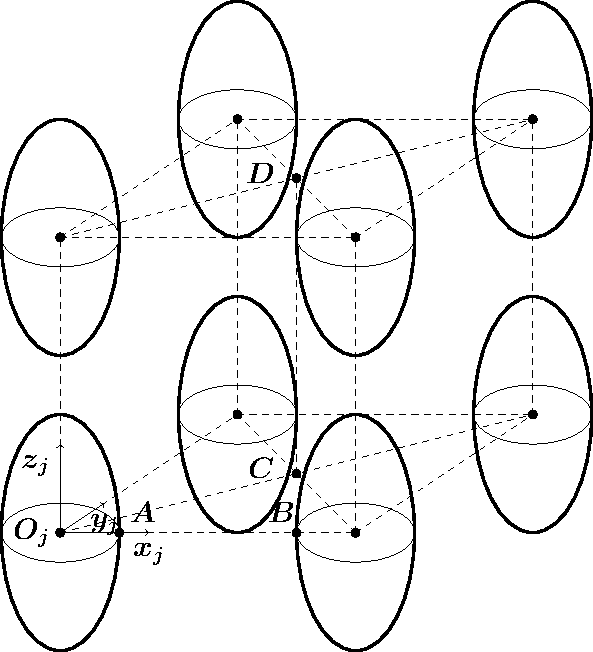
\includegraphics[width=8cm]{cartesian-spheroids.pdf}
\caption{Схематическое представление задачи}
\label{f:9:1}
\end{figure}

Введем вытянутые сфероидальные системы координат $(\xi_j,\eta_j,\varphi_j)$, совмещенные с цилиндрическими системами. Все введенные системы координат связаны соотношениями 

\begin{equation}
\left\{ {\begin{array}{*{20}{l}}
{{x_j} = {x_\alpha} + {x_{j\alpha}},}\\
{{y_j} = {y_\alpha} + {y_{j\alpha}},}\\
{{z_j} = {z_\alpha} + {z_{j\alpha}};}
\end{array}} \right.
\end{equation}

\begin{multline}
{x_i} = {\rho _i}\cos {\varphi _i} = {r_i}\sin {\theta _i}\cos {\varphi _i} = {c_i}{\mathop{\rm sh}\nolimits} {\xi _i}\sin {\eta _i}\cos {\varphi _i} = \\
= {\tilde c_i}{\mathop{\rm ch}\nolimits} {\tilde \xi _i}\sin {\tilde \eta _i}\cos {\varphi _i},
\end{multline}

\begin{multline}
{y_i} = {\rho _i}\sin {\varphi _i} = {r_i}\sin {\theta _i}\sin {\varphi _i} = {c_i}{\mathop{\rm sh}\nolimits} {\xi _i}\sin {\eta _i}\sin {\varphi _i} = \\
= {\tilde c_i}{\mathop{\rm ch}\nolimits} {\tilde \xi _i}\sin {\tilde \eta _i}\sin {\varphi _i},
\end{multline}

\begin{equation}
{z_i} = {r_i}\cos {\theta _i} = {c_i}{\mathop{\rm ch}\nolimits} {\xi _i}\cos {\eta _i} = {\tilde c_i}{\mathop{\rm sh}\nolimits} {\tilde \xi _i}\cos {\tilde \eta _i},
\end{equation}

\noindent где ${x_i},{y_i},{z_i} \in \left( { - \infty ;\infty } \right)$; ${\rho _i},{r_i},{\xi _i} \in \left[ {\left. {0;\infty } \right)} \right.$; ${\eta _i} \in \left[ {0;\pi } \right]$; ${\tilde \xi _i} \in \left( { - \infty ,\infty } \right)$; ${\tilde \eta _i} \in \left[ {0;\dfrac{\pi }{2}} \right]$; $\varphi  \in \left[ {0;2\pi } \right]$; ${c_i},{\tilde c_i}$ $\left( {{c_i},{{\tilde c}_i} > 0} \right)$~--- параметры сфероидальных систем координат.


В сфероидальных координатах поверхности полостей задаются уравнениями $\Gamma_j:\,\xi_j=\xi_{j0}$, где $\xi_{j0}$ можно найти из системы уравнений

\begin{equation}
\left\{ {\begin{array}{*{20}{l}}
{{c_j}{\mathop{\rm sh}\nolimits} {\xi _{j0}} = {d_{j1}},}\\
{{c_j}{\mathop{\rm ch}\nolimits} {\xi _{j0}} = {d_{j2}}.}
\end{array}} \right.
\end{equation}

Для определения НДС в рассматриваемом теле необходимо решить краевую задачу относительно вектора перемещения $\mathbf{U}$, удовлетворяющего уравнению Ламе, граничным условиям на поверхностях $\Gamma_j$

\begin{equation}
{\bf{FU}}{|_{{\Gamma _j}}} = 0\qquad {\kern 1pt} \left( {j = \overline {1,N} } \right)
\label{eq:9:4}
\end{equation}

\noindent и условиям на бесконечности

\begin{equation}
{\bf{FU}}{|_{z =  \pm \infty }} =  \pm T{{\bf{e}}_z}\quad\text{(одноосное растяжение)},
\label{eq:9:21}
\end{equation}

\begin{equation}
{\bf{FU}}{|_{\rho  = \infty }} = T{{\bf{e}}_\rho }\quad\text{(двуосное растяжение)}.
\label{eq:9:22}
\end{equation}

Решение задачи будем искать в виде

\begin{equation}
{\bf{U}} = {\bf{\tilde U}} + {{\bf{U}}_0},
\end{equation}

\begin{equation}
{\bf{\tilde U}} = \sum\limits_{j = 1}^N {\sum\limits_{s = 1}^3 {\sum\limits_{n = 0}^\infty  {\sum\limits_{m =  - n - 1}^{n + 1} {a_{s,n,m}^{(j)}} } } } {\bf{U}}_{s,n,m}^{ + (5)}\left( {{\xi _j},{\eta _j},{\varphi _j}} \right),
\end{equation}

\noindent где $a_{s,n,m}^{(j)}$~--- неизвестные коэффициенты;

\begin{equation}
{{\bf{U}}_0} = \frac{T}{{2G}}\left( { - \frac{\sigma }{{1 + \sigma }}{\rho _1}{{\bf{e}}_{{\rho _1}}} + \frac{1}{{1 + \sigma }}{z_1}{{\bf{e}}_z}} \right)\,\text{(одноосное растяжение)};
\label{eq:9:7}
\end{equation}

\begin{equation}
{{\bf{U}}_0} = \frac{T}{{2G}}\left( {\frac{{1 - \sigma }}{{1 + \sigma }}{\rho _1}{{\bf{e}}_{{\rho _1}}} - \frac{{2\sigma }}{{1 + \sigma }}{z_1}{{\bf{e}}_z}} \right)\quad\text{(двуосное растяжение)}.
\label{eq:9:8}
\end{equation}

В работе~\cite{Nikolaev2011} были введены следующие частные решения уравнения Ламе во внешности (внутренности) вытянутого сфероида $\Omega _5^ \pm \left\{ {(\xi ,\eta ,\varphi ):{\mkern 1mu} {\kern 1pt} \xi  \mathbin{\lower.3ex\hbox{$\buildrel>\over
{\smash{\scriptstyle<}\vphantom{_x}}$}} {\xi _0}} \right\}$:

\begin{multline}
{\bf{U}}_{s,n,m}^{ \pm (5)}\left( {\xi ,\eta ,\varphi } \right) = \\
= \frac{c}{{2n + 1}}{{\bf{D}}_s}\left[ {u_{n - 1,m}^{ \pm (5)}\left( {\xi ,\eta ,\varphi } \right) - u_{n + 1,m}^{ \pm (5)}\left( {\xi ,\eta ,\varphi } \right)} \right];\quad {\kern 1pt} s = 1,3;
\label{eq:9:1}
\end{multline}

\begin{equation}
{\bf{U}}_{2,n,m}^{ \pm (5)}\left( {\xi ,\eta ,\varphi } \right) = {{\bf{D}}_2}u_{n,m}^{ \pm (5)}\left( {\xi ,\eta ,\varphi } \right) - c{{\mathop{\rm ch}\nolimits} ^2}{\xi _0}{{\bf{D}}_1}u_{n \pm 1,m}^{ \pm (5)}\left( {\xi ,\eta ,\varphi } \right),
\label{eq:9:2}
\end{equation}

\noindent где $n=0,1,\dots$, $|m|\le n+1$;

\begin{multline}
u_{n,m}^{ \pm (5)}\left( {\xi ,\eta ,\varphi } \right) = \\
= \left\{ \begin{array}{l}
Q_n^{ - m}({\mathop{\rm ch}\nolimits} \xi )\\
P_n^{ - m}({\mathop{\rm ch}\nolimits} \xi )
\end{array} \right\}P_n^m(\cos \eta ){e^{im\varphi }},\quad n,m \in \mathbb{Z}, |m| \le n;
\end{multline}

\noindent где $P_n^m(x)$, $Q_n^m(x)$~--- функции Лежандра первого и второго рода соответственно;

\begin{equation}
{{\bf{D}}_1} = \nabla  = {{\bf{e}}_x}\frac{\partial }{{\partial x}} + {{\bf{e}}_y}\frac{\partial }{{\partial y}} + {{\bf{e}}_z}\frac{\partial }{{\partial z}};
\label{eq:9:23a}
\end{equation}
\begin{equation}
{{\bf{D}}_2} = z\nabla  - \chi {{\bf{e}}_z};
\label{eq:9:23b}
\end{equation}
\begin{equation}
{{\bf{D}}_3} = i\left[ {\nabla  \times {{\bf{e}}_z}} \right].
\label{eq:9:23c}
\end{equation}

В развернутой координатной форме формулы~\eqref{eq:9:1}, \eqref{eq:9:2} имеют вид:

\begin{equation}
{\bf{U}}_{1,n,m}^{ \pm (5)} = u_{n,m - 1}^{ \pm (5)}{{\bf{e}}_{ - 1}} - u_{n,m + 1}^{ \pm (5)}{{\bf{e}}_1} - u_{n,m}^{ \pm (5)}{{\bf{e}}_0};
\end{equation}

\begin{multline}
{\bf{U}}_{2,n,m}^{ \pm (5)} = qu_{1,n,m - 1}^{ \pm (5)}{{\bf{e}}_{ - 1}} - qu_{1,n,m + 1}^{ \pm (5)}{{\bf{e}}_1} - \left[ {qu_{1,n,m}^{ \pm (5)} + \chi u_{n,m}^{ \pm (5)}} \right]{{\bf{e}}_0} + \\
+c\left( {{q^2} - q_0^2} \right)\nabla u_{n \pm 1,m}^{ \pm (5)};
\end{multline}

\begin{equation}
{\bf{U}}_{3,n,m}^{ \pm (5)} =  - u_{n,m - 1}^{ \pm (5)}{{\bf{e}}_{ - 1}} - u_{n,m + 1}^{ \pm (5)}{{\bf{e}}_1}.
\end{equation}

Здесь использованы обозначения
	
\begin{equation}
u_{1,n,m}^{ \pm (5)} = u_{1,n,m}^ \pm (\xi )P_n^m(\cos \eta ){e^{im\varphi }};
\end{equation}
\begin{equation}
u_{1,n,m}^ \pm (\xi ) = \left\{ \begin{array}{l}
(n + m + 1)Q_{n + 1}^{ - m}(q)\\
 - (n - m)P_{n - 1}^{ - m}(q)
\end{array} \right\};
\end{equation}

\begin{equation}
q = {\mathop{\rm ch}\nolimits} \xi ,\quad {q_0} = {\mathop{\rm ch}\nolimits} {\xi _0},\quad {{\bf{e}}_{ \mp 1}} = \frac{1}{2}\left( {{{\bf{e}}_x} \pm i{{\bf{e}}_y}} \right),\quad {{\bf{e}}_0} = {{\bf{e}}_z}.
\end{equation}

В работе~\cite{Nikolaev1998} введено понятие базисности системы решений уравнения Ламе в односвязной канонической области и доказана базисность решений~\eqref{eq:9:1}, \eqref{eq:9:2} в соответствующих областях $\Omega_5^\pm$.{\sloppy\par}

Относительно перемещения $\mathbf{\tilde U}$ граничные условия можно записать так:

\begin{equation}
{\bf{F\tilde U}}{|_{{\Gamma _j}}} =  - {\bf{F}}{{\bf{U}}_0}{|_{{\Gamma _j}}}.
\end{equation}

На бесконечности вектор $\mathbf{F\tilde U}$ подчиняется условиям~\eqref{eq:8:3}, \eqref{eq:8:4}. Заметим, что вектор усилий ${\bf{F}}{{\bf{U}}_0}{|_{{\Gamma _j}}}$ для каждого типа растяжений упругого пространства находят по формулам $(\mathbf{n}_j=\mathbf{e}_{\xi_j})$

\begin{equation}
{\bf{F}}{{\bf{U}}_0}{|_{{\Gamma _j}}} = T{H_j}{\mathop{\rm sh}\nolimits} {\xi _{j0}}{P_1}(\cos {\eta _j}){{\bf{e}}_z}\quad\text{(одноосное растяжение)},
\end{equation}

\begin{equation}
{\bf{F}}{{\bf{U}}_0}{|_{{\Gamma _j}}} =  - T{H_j}{\mathop{\rm ch}\nolimits} {\xi _{j0}}P_1^{(1)}(\cos {\eta _j}){{\bf{e}}_{{\rho _j}}}\quad\text{(двуосное растяжение)},
\end{equation}

\noindent где ${H_j} = {\left( {{{{\mathop{\rm ch}\nolimits} }^2}{\xi _{j0}} - {{\cos }^2}{\eta _j}} \right)^{ - \frac{1}{2}}}$.

Используя теоремы сложения, перемещение $\mathbf{\tilde U}$ можно записать в системе координат с началом в точке $O_j$:

\begin{multline}
{\bf{\tilde U}} = \sum\limits_{s = 1}^3 {\sum\limits_{n = 0}^\infty  {\sum\limits_{m =  - n - 1}^{n + 1} {a_{s,n,m}^{(j)}} } } {\bf{U}}_{s,n,m}^{ + (5)}\left( {{\xi _j},{\eta _j},{\varphi _j}} \right) + \\
+ \sum\limits_{n = 0}^\infty  {\sum\limits_{m =  - n - 1}^{n + 1} {\left\{ {{\bf{U}}_{1,n,m}^{ - (5)}\left( {{\xi _j},{\eta _j},{\varphi _j}} \right)\sum\limits_{\alpha  \ne j} {\sum\limits_{k = 0}^\infty  {\sum\limits_{l =  - k - 1}^{k + 1} {\left[ {a_{1,k,l}^{(\alpha )}f_{k,l,j,\alpha }^{ - (55)n,m} + } \right.} } } } \right.} } \\
\left. { + a_{2k,l}^{(\alpha )}\tilde f_{k,l,j,\alpha }^{ - (55)n,m}} \right] + {\bf{U}}_{2,n,m}^{ - (5)}\left( {{\xi _j},{\eta _j},{\varphi _j}} \right)\sum\limits_{\alpha  \ne j} {\sum\limits_{k = 0}^\infty  {\sum\limits_{l =  - k - 1}^{k + 1} {a_{2,k,l}^{(\alpha )}} } \tilde f_{k,l,j,\alpha }^{ - (55)n,m} + } \\
\left. { + {\bf{U}}_{3,n,m}^{ - (5)}\left( {{\xi _j},{\eta _j},{\varphi _j}} \right)\sum\limits_{\alpha  \ne j} {\sum\limits_{k = 0}^\infty  {\sum\limits_{l =  - k - 1}^{k + 1} {a_{3,k,l}^{(\alpha )}} } f_{k,l,j,\alpha }^{ - (55)n,m}} } \right\};
\label{eq:9:3}
\end{multline}

\begin{equation}
f_{n,m,j,\alpha}^{ - (55)k,l} = \sum\limits_{r = k}^\infty  {f_{n,m,j,\alpha}^{(54)r,l}({c_\alpha})g_{r,l}^{ - (45)k}} ({c_j});
\label{eq:9:10}
\end{equation}

\begin{equation}
g_{k,l}^{ - (45)s}({c_j}) = \sqrt \pi  {\varepsilon _{ks}}{\left( {\dfrac{{{c_j}}}{2}} \right)^k}\dfrac{{s + \dfrac{1}{2}}}{{\Gamma \left( {\dfrac{k}{2} - \dfrac{s}{2} + 1} \right)\Gamma \left( {\dfrac{k}{2} + \dfrac{s}{2} + \dfrac{3}{2}} \right)}},
\label{eq:9:11}
\end{equation}

\begin{multline}
f_{n,m,j,\alpha}^{(54)r,l}({c_\alpha}) = \\
= \sum\limits_{p = 0}^\infty  {{{( - 1)}^{p + l + m}}} \sqrt \pi  {\left( {\frac{{{c_\alpha}}}{2}} \right)^{p + 1}}\frac{{{\varepsilon _{pn}}u_{p + r,m - l}^{ + (4)}\left( {{r_{j\alpha}},{\theta _{j\alpha}},{\varphi _{j\alpha}}} \right)}}{{\Gamma \left( {\frac{{p - n}}{2} + 1} \right)\Gamma \left( {\frac{{p + n}}{2} + \frac{3}{2}} \right)}};
\label{eq:9:12}
\end{multline}

\begin{multline}
\tilde f_{n,m,j,\alpha}^{ - (55)k,l} = \sum\limits_{r = k}^\infty  \bigg[ {c_\alpha}q_{\alpha 0}^2f_{n + 1,m,j,\alpha}^{(54)r + 1,l}({c_\alpha})g_{r,l}^{ - (45)k}({c_j}) + \\ 
+ {z_{j\alpha}}f_{n,m,j,\alpha}^{(54)r + 1,l}({c_\alpha})g_{r,l}^{ - (45)k}({c_j}) - \\
- {c_j}q_{j0}^2\frac{{2k + 1}}{{2k + 3}}f_{n,m,j,\alpha}^{(54)r,l}({c_\alpha})g_{r - 1,l}^{ - (45)k + 1}({c_j}) \bigg],
\label{eq:9:13}
\end{multline}

%\begin{equation}
%f_{n,m,\alpha ,\beta }^{ + (55)k,l} = \sum\limits_{j = n}^\infty  {g_{n,m}^{ + (54)j}} ({c_\alpha })f_{j,m,\alpha ,\beta }^{(45)k,l}({c_\beta });
%\label{eq:9:10}
%\end{equation}
%
%\begin{equation}
%g_{n,m}^{ + (54)j}({c_\alpha }) = {( - 1)^m}\sqrt \pi  {\left( {\frac{{{c_\alpha }}}{2}} \right)^{j + 1}}\frac{{{\varepsilon _{jn}}}}{{\Gamma \left( {\frac{{j - n}}{2} + 1} \right)\Gamma \left( {\frac{{j + n}}{2} + \frac{3}{2}} \right)}};
%\label{eq:9:11}
%\end{equation}
%
%\begin{multline}
%f_{j,m,\alpha ,\beta }^{(45)k,l}({c_\beta }) = \\ 
%= \sum\limits_{p = 0}^\infty  {{{( - 1)}^{p + l}}} \sqrt \pi  {\left( {\frac{{{c_\beta }}}{2}} \right)^p}\frac{{{\varepsilon _{pk}}\left( {k + \frac{1}{2}} \right)u_{j + p,m - l}^{ + (4)}\left( {{r_{\alpha \beta }},{\theta _{\alpha \beta }},{\varphi _{\alpha \beta }}} \right)}}{{\Gamma \left( {\frac{{p - k}}{2} + 1} \right)\Gamma \left( {\frac{{p + k}}{2} + \frac{3}{2}} \right)}};
%\label{eq:9:12}
%\end{multline}
%
%\begin{multline}
%\tilde f_{n,m,\alpha ,\beta }^{ + (55)k,l} = \sum\limits_{j = n}^\infty  {\left[ {{c_\beta }q_{\beta 0}^2\frac{{2k + 1}}{{2k + 3}}g_{n,m}^{ + (54)j}({c_\alpha })f_{j + 1,m,\alpha ,\beta }^{(45)k + 1,l}({c_\beta }) + } \right.} \\
%\left. { + {z_{\alpha \beta }}g_{n,m}^{ + (54)j}({c_\alpha })f_{j + 1,m,\alpha ,\beta }^{(45)k,l}({c_\beta })\frac{{}}{{}}{c_\alpha }q_{\alpha 0}^2g_{n + 1,m}^{ + (54)j - 1}({c_\alpha })f_{j,m,\alpha ,\beta }^{(45)k,l}({c_\beta })} \right].
%\label{eq:9:13}
%\end{multline}

Формулы для напряжений, отвечающих базисным вектор-функциям перемещений $\mathbf{U}_{s,n,m}^{\pm(5)}(\xi_j,\eta_j,\varphi_j)$ на поверхностях $\Gamma_j$ ($\mathbf{n}_j=\mathbf{e}_{\xi_j}$~--- нормаль к поверхности  $\Gamma_j$):

\begin{multline}
{\bf{FU}}_{1,n,m}^{ \pm (5)}\left( {{\xi _j},{\eta _j},{\varphi _j}} \right) = 2G\frac{{{H_j}}}{{{c_j}}}\left[ {\frac{\partial }{{\partial {\xi _j}}}u_{n,m - 1}^{ \pm (5)}\left( {{\xi _j},{\eta _j},{\varphi _j}} \right){{\bf{e}}_{ - 1}} - } \right.\\
- \frac{\partial }{{\partial {\xi _j}}}u_{n,m + 1}^{ \pm (5)}\left( {{\xi _j},{\eta _j},{\varphi _j}} \right){{\bf{e}}_1}\left. { - \frac{\partial }{{\partial {\xi _j}}}u_{n,m}^{ \pm (5)}\left( {{\xi _j},{\eta _j},{\varphi _j}} \right){{\bf{e}}_0}} \right];
\label{eq:9:f1}
\end{multline}

\begin{multline}
{\bf{FU}}_{2,n,m}^{ \pm (5)}\left( {{\xi _j},{\eta _j},{\varphi _j}} \right) = 2G\frac{{{H_j}}}{{{c_j}}}\left\{ {\left[ {q_j^2\frac{\partial }{{\partial {\xi _j}}}\left( {\frac{{u_{1,n,m - 1}^{ \pm (5)}}}{{{q_j}}}} \right) - 2\sigma u_{2,n,m}^{ \pm (5)}} \right]{{\bf{e}}_{ - 1}} - } \right.\\
- \left[ {q_j^2\frac{\partial }{{\partial {\xi _j}}}\left( {\frac{{u_{1,n,m + 1}^{ \pm (5)}}}{{{q_j}}}} \right) - 2\sigma u_{3,n,m}^{ \pm (5)}} \right]{{\bf{e}}_1} - \left[ {q_j^2\frac{\partial }{{\partial {\xi _j}}}\left( {\frac{{u_{1,n,m}^{ \pm (5)}}}{{{q_j}}}} \right) + } \right.\\
\left. { + \left. {(1 - 2\sigma )\frac{\partial }{{\partial {\xi _j}}}u_{n,m}^{ \pm (5)}} \right]{{\bf{e}}_0}} \right\};
\label{eq:9:f2}
\end{multline}

\begin{multline}
{\bf{FU}}_{3,n,m}^{ \pm (5)}\left( {{\xi _j},{\eta _j},{\varphi _j}} \right) = 2G\frac{{{H_j}}}{{{c_j}}}\left\{ { - \left[ {\frac{\partial }{{\partial {\xi _j}}}u_{n,m - 1}^{ \pm (5)} - \frac{1}{2}u_{2,n,m}^{ \pm (5)}} \right]{{\bf{e}}_{ - 1}} - } \right.\\
\left. { - \left[ {\frac{\partial }{{\partial {\xi _j}}}u_{n,m + 1}^{ \pm (5)} - \frac{1}{2}u_{3,n,m}^{ \pm (5)}} \right]{{\bf{e}}_1} + \frac{m}{2}\frac{{{q_j}}}{{{{\bar q}_j}}}u_{n,m}^{ \pm (5)}{{\bf{e}}_0}} \right\},
\label{eq:9:f3}
\end{multline}

\noindent где ${H_j} = {\left( {q_j^2 - {{\cos }^2}{\eta _j}} \right)^{ - \frac{1}{2}}}$;

\begin{equation}
u_{1,n,m}^{ \pm (5)}\left( {{\xi _j},{\eta _j},{\varphi _j}} \right) = \tilde u_{1,n,m}^{ \pm (5)}({\xi _j})P_n^m(\cos {\eta _j}){e^{im{\varphi _j}}};
\end{equation}

\begin{equation}
u_{2,n,m}^{ \pm (5)}\left( {{\xi _j},{\eta _j},{\varphi _j}} \right) = \tilde u_{2,n,m}^{ \pm (5)}({\xi _j})P_n^{m - 1}(\cos {\eta _j}){e^{i(m - 1){\varphi _j}}};
\end{equation}

\begin{equation}
u_{3,n,m}^{ \pm (5)}\left( {{\xi _j},{\eta _j},{\varphi _j}} \right) = \tilde u_{n,m}^{ \pm (5)}({\xi _j})P_n^{m + 1}(\cos {\eta _j}){e^{i(m + 1){\varphi _j}}};
\end{equation}

\begin{equation}
\tilde u_{n,m}^{ \pm (5)}(\xi ) = \left\{ \begin{array}{l}
Q_n^{ - m}(q)\\
P_n^{ - m}(q)
\end{array} \right\};
\end{equation}
\begin{equation}
\tilde u_{1,n,m}^{ \pm (5)}(\xi ) = \left\{ \begin{array}{l}
(n + m + 1)Q_{n + 1}^{ - m}(q)\\
 - (n - m)P_{n - 1}^{ - m}(q)
\end{array} \right\};
\end{equation}

\begin{equation}
\tilde u_{2,n,m}^{ \pm (5)}(\xi ) = (n + m)(n - m + 1)\tilde u_{n,m}^{ \pm (5)}(\xi ),\qquad {\kern 1pt} q = {\mathop{\rm ch}\nolimits} \xi ,\quad \bar q = {\mathop{\rm sh}\nolimits} \xi.
\end{equation}

После перехода в формуле~\eqref{eq:9:3} к напряжениям и удовлетворения граничных условий относительно неизвестных $a_{s,n,m}^{(j)}$ получаем бесконечную систему линейных алгебраических уравнений:

\begin{multline}
\sum\limits_{s = 1}^3 {a_{s,n,m}^{(j)}} W_{s,n,m}^{ + (k)}({\xi _{j0}}) + W_{1,n,m}^{ - (k)}({\xi _{j0}})\sum\limits_{\alpha  \ne j} {\sum\limits_{k = 0}^\infty  {\sum\limits_{l =  - k - 1}^{k + 1} {\left[ {a_{1,k,l}^{(\alpha )}f_{k,l,j,\alpha }^{ - (55)n,m} + } \right.} } } \\
\left. { + a_{2,k,l}^{(\alpha )}\tilde f_{k,l,j,\alpha }^{ - (55)n,m}} \right] + W_{2,n,m}^{ - (k)}({\xi _{j0}})\sum\limits_{\alpha  \ne j} {\sum\limits_{k = 0}^\infty  {\sum\limits_{l =  - k - 1}^{k + 1} {a_{2,k,l}^{(\alpha )}} } f_{k,l,j,\alpha }^{ - (55)n,m} + } \\
+ W_{3,n,m}^{ - (k)}({\xi _{j0}})\sum\limits_{\alpha  \ne j} {\sum\limits_{k = 0}^\infty  {\sum\limits_{l =  - k - 1}^{k + 1} {a_{3,k,l}^{(\alpha )}} } f_{k,l,j,\alpha }^{ - (55)n,m} = 0;}
\label{eq:9:24}
\end{multline}

$$
n,m \in\mathbb{Z}:\quad n \ge 0,\quad |m| \le n + 1,\quad k =  - 1,{\mkern 1mu} {\kern 1pt} 0,{\mkern 1mu} {\kern 1pt} 1;
$$

\begin{equation}
W_{1,n,m}^{ \pm ( - 1)}(\xi ) = \frac{\partial }{{\partial \xi }}\tilde u_{n,m - 1}^{ \pm (5)}(\xi ),\quad W_{1,n,m}^{ \pm (1)} =  - \frac{\partial }{{\partial \xi }}\tilde u_{n,m + 1}^{ \pm (5)}(\xi );
\label{eq:9:15}
\end{equation}

\begin{multline}
W_{1,n,m}^{ \pm (0)}(\xi ) =  - \frac{\partial }{{\partial \xi }}\tilde u_{n,m}^{ \pm (5)}(\xi ); \\
W_{2,n,m}^{ \pm ( - 1)}(\xi ) = {q^2}\frac{\partial }{{\partial \xi }}\left[ {\frac{{\tilde u_{1,n,m - 1}^{ \pm (5)}(\xi )}}{q}} \right] - 2\sigma \tilde u_{2,n,m}^{ \pm (5)}(\xi );
\label{eq:9:16}
\end{multline}

\begin{equation}
W_{2,n,m}^{ \pm (1)}(\xi ) =  - {q^2}\frac{\partial }{{\partial \xi }}\left[ {\frac{{u_{1,n,m + 1}^{ \pm (5)}(\xi )}}{q}} \right] + 2\sigma \tilde u_{n,m}^{ \pm (5)}(\xi );
\label{eq:9:17}
\end{equation}

\begin{equation}
W_{2,n,m}^{ \pm (0)}(\xi ) =  - {q^2}\frac{\partial }{{\partial \xi }}\left[ {\frac{{\tilde u_{1,n,m}^{ \pm (5)}(\xi )}}{q}} \right] - (1 - 2\sigma )\frac{\partial }{{\partial \xi }}\tilde u_{n,m}^{ \pm (5)}(\xi );
\label{eq:9:18}
\end{equation}

\begin{equation}
W_{3,n,m}^{ \pm ( - 1)}(\xi ) =  - \frac{\partial }{{\partial \xi }}\tilde u_{n,m - 1}^{ \pm (5)}(\xi ) + \frac{1}{2}\tilde u_{2,n,m}^{ \pm (5)}(\xi );
\label{eq:9:19}
\end{equation}

\begin{equation}
W_{3,n,m}^{ \pm (1)}(\xi ) =  - \frac{\partial }{{\partial \xi }}\tilde u_{n,m + 1}^{ \pm (5)}(\xi ) + \frac{1}{2}\tilde u_{n,m}^{ \pm (5)}(\xi );
\label{eq:9:20a}
\end{equation}
\begin{equation}
W_{3,n,m}^{ \pm (0)}(\xi ) = \frac{m}{2}\frac{q}{{\bar q}}\tilde u_{n,m}^{ \pm (5)}(\xi );
\label{eq:9:20b}
\end{equation}

\begin{equation}
W_{n,m}^{(k)j} = \left\{ \begin{array}{l}
 - \dfrac{T}{{2G}}{c_j}{\mathop{\rm sh}\nolimits} {\xi _{j0}}{\delta _{n1}}{\delta _{m0}}{\delta _{k0}}\quad\text{(одноосное растяжение)},\\
 \\
\dfrac{T}{{2G}}{c_j}{\mathop{\rm ch}\nolimits} {\xi _{j0}}{\delta _{n1}}{\delta _{m0}}{\delta _{k1}}\quad\text{(двуосное растяжение)}.
\end{array} \right.
\label{eq:9:14}
\end{equation}

\section{Анализ разрешающей системы}

\begin{theorem}
При выполнении условия ${\xi _{j0}} < \xi _j^*$ оператор системы~\eqref{eq:9:24} является фредгольмовым в гильбертовом пространстве $l_2$.
\end{theorem}

\begin{proof}
Путем переобозначения неизвестных коэффициентов

\begin{equation}
\tilde a_{s,n,m}^{(j)} = a_{s,n,m}^{(j)}Q_n^{ - m}({q_{j0}})\sqrt {\frac{{(n + m)!}}{{(n + 1/2)(n - m)!}}}
\end{equation}
и разрешения системы относительно $\tilde a_{s,n,m}^{(j)}$ можно представить систему~\eqref{eq:9:24} в виде

\begin{equation}
\tilde a_{s,n,m}^{(j)} + \sum\limits_{\alpha\neq j}\sum\limits_{p = 1}^3 {\sum\limits_{k = 0}^\infty  {\sum\limits_{l =  - k - 1}^{k + 1} {T_{j,s,n,m}^{\alpha,p,k,l}} } } \tilde a_{p,k,l}^{(\alpha)} = W_{s,n,m}^{(j)},
\label{eq:9:25}
\end{equation}
$$n,m \in\mathbb{Z},\quad n \ge 0,\quad |m| \le n + 1;\quad s = 1,2,3;\quad j = \overline{1,N}.$$

Ввиду громоздкости опустим явную запись матричных коэффициентов системы~\eqref{eq:9:25}. Заметим, однако, что модуль матричных коэффициентов $\left|T_{j,s,n,m}^{\alpha,p,k,l}\right|$ можно оценить сверху конечными линейными комбинациями выражений вида

\begin{equation}
{n^\gamma }{k^\beta }{\left| {\frac{{P_n^{ - m}\left( {{q_{j0}}} \right)}}{{Q_k^{ - l}\left( {{q _{\alpha 0}}} \right)}}} \right|^2}\frac{{(n + m)!(k + l)!}}{{(n - m)!(k - l)!}}{\left| {f_{k,l,j,\alpha}^{-(55)n,m}} \right|^2},
\label{eq:9:26}
\end{equation}
где $\beta$ и $\gamma$~--- заданные числа, не зависящие от $n$, $k$, $l$, $m$.

Оценим сходимость ряда

\begin{multline}
\sum\limits_{n = 0}^\infty\sum\limits_{m =  - n}^n\sum\limits_{k = 0}^\infty  \sum\limits_{l =  - k}^k{{\left[ {\frac{{{n^\gamma }{k^\beta }P_n^{ - m}({q_{j0}})}}{{Q_k^{ - l}\left( {{q _{\alpha 0}}} \right)}}} \right]}^2}\times \\
\times\frac{{(n + m)!(k + l)!}}{{(n - m)!(k - l)!}}{{\left| {f_{k,l,j,\alpha}^{-(55)n,m}} \right|}^2}.   
\label{eq:9:27}
\end{multline}

С этой целью рассмотрим теорему сложения гармонических функций~\eqref{eq:1:22}, которую можно записать так:

\begin{equation}
u_{n,m}^{ + (5)}\left( {{\xi _{\alpha}},{\eta _{\alpha}},{\varphi _{\alpha}}} \right) = \sum\limits_{k = 0}^\infty\sum\limits_{l=-k}^k f_{n,m,j,\alpha}^{-(55)k,l} u_{k,l}^{ - (5)}\left( {{\xi _j},{\eta _j},{\varphi _j}} \right).
\label{eq:9:28}
\end{equation}

Равенство~\eqref{eq:9:28} представляет собой разложение функции, входящей в ее левую часть, в ряд Фурье по ортонормированной системе функций $\sqrt {(k + 1/2)\frac{{(k - l)!}}{{(k + l)!}}} P_k^l(\cos {\eta _j})\frac{1}{{\sqrt {2\pi } }}{e^{il{\varphi _j}}}$ на поверхности сфероида. Для этого разложения справедливо равенство Парсеваля\sloppy

\begin{multline}
\frac{1}{{2\pi }}\int\limits_0^{2\pi } {\int\limits_0^\pi  {{{\left| {u_{n,m}^{ + (5)}\left( {{\xi _{\alpha}},{\eta _{\alpha}},{\varphi _{\alpha}}} \right)} \right|}^2}} } \sin {\eta _j}d{\eta _j}d{\varphi _j} = \\
= \sum\limits_{k = 0}^\infty  {\sum\limits_{l =  - k}^k {{{\left| {f_{n,m,j,\alpha}^{-(55)k,l}} \right|}^2}} } {\left| {P_k^{ - l}({q_{j0}})} \right|^2}\frac{{(k + l)!}}{{(k - l)!(k + 1/2)}}.
\label{eq:9:29}
\end{multline}

Положим в формуле~\eqref{eq:9:29} $\xi_j=\xi_{0j}$, после чего помножим обе части равенства~\eqref{eq:9:29} на выражение $\dfrac{{(n + m)!}}{{(n - m)!}}{{{{\left| {Q_n^{ - m}\left( {{q _{\alpha 0}}} \right)} \right|}^{-2}}}}$ и просуммируем по $n$ и $m$ от $0$ до $\infty$ и от $-n$ до $n$ соответственно. В результате получим

\begin{multline}
\frac{1}{{2\pi }}\int\limits_0^{2\pi } {\int\limits_0^\pi  {\sum\limits_{n = 0}^\infty  {\sum\limits_{m =  - n}^n {{{\left| {\frac{{Q_n^{ - m}\left( {{q _{\alpha}}} \right)}}{{Q_n^{ - m}\left( {{q _{\alpha 0}}} \right)}}} \right|}^2}} } } } \frac{1}{{n + \frac{1}{2}}}\frac{{{{\left| {P_n^m(\cos {\eta _{\alpha}})} \right|}^2}}}{{||P_n^m|{|^2}}}\sin {\eta _j}d{\eta _j}d{\varphi _j} = \\
= \sum\limits_{n = 0}^\infty  {\sum\limits_{m =  - n}^n {\sum\limits_{k = 0}^\infty  {\sum\limits_{l =  - k}^k {{{\left| {\frac{{P_k^{ - l}({q_{j0}})}}{{Q_n^{ - m}\left( {{q _{\alpha 0}}} \right)}}} \right|}^2}} } } } \times \\
\times\frac{{(n + m)!}}{{(n - m)!}}\frac{{(k + l)!}}{{(k - l)!}}\frac{1}{{\left( {n + \frac{1}{2}} \right)\left( {k + \frac{1}{2}} \right)}}{\left| {f_{n,m}^{-(55)k,l}} \right|^2}.
\label{eq:9:30}
\end{multline}

Ряд в левой части равенства~\eqref{eq:9:30} сходится при условии $\xi_{\alpha}>\xi_{\alpha 0}$. Найдем наименьшее значение $\xi_{\alpha}$, при котором точка с координатами $\left( {{\xi _{\alpha}},{\eta _{\alpha}},{\varphi _{\alpha}}} \right)$ находится на поверхности сфероида $\xi_j=\xi_{j0}$. Очевидно, это значение $\xi_{\alpha}$ соответствует случаю, когда сфероиды $\xi_j=\xi_{j0}$ и $\xi_{\alpha}=\xi_{\alpha 0}$ касаются. Обозначим это значение переменной $\xi_{\alpha}$ через $\xi_{\alpha}^*$. Оно может быть найдено из решения задачи касания двух сфероидов по формуле

\begin{equation}
{{\mathop{\rm ch}\nolimits} ^2}\xi _j^* = \frac{{\sin {\eta _\alpha}{\mathop{\rm ch}\nolimits} {\xi _{\alpha 0}}\left( {{c_\alpha}{\mathop{\rm ch}\nolimits} {\xi _{\alpha 0}}\cos {\eta _\alpha} + {z_{j\alpha}}} \right)}}{{{c_\alpha}\sin {\eta _\alpha}\cos {\eta _\alpha} + \sin {\eta _\alpha}{\mathop{\rm ch}\nolimits} {\xi _{\alpha 0}}{z_{j\alpha}} + \cos {\eta _\alpha}{\mathop{\rm sh}\nolimits} {\xi _{\alpha 0}}{\rho _{j\alpha}}}},
\end{equation}
где $\eta_\alpha\in[0,\pi]$~--- тот корень уравнения

\begin{multline}
\left( {{c_\alpha}{\mathop{\rm ch}\nolimits} {\xi _{\alpha 0}}{\mathop{\rm sh}\nolimits} {\xi _{\alpha 0}} - {\mathop{\rm ch}\nolimits} {\xi _{\alpha 0}}{\rho _{j\alpha}}\sin {\eta _\alpha}{\mathop{\rm sh}\nolimits} {\xi _{\alpha 0}}{z_{j\alpha}}\cos {\eta _\alpha}} \right)\left( {{c_\alpha}\sin {\eta _\alpha}\cos {\eta _\alpha} + } \right.\\
\left. { + {\mathop{\rm ch}\nolimits} {\xi _{\alpha 0}}{z_{j\alpha}}\sin {\eta _\alpha} + {\mathop{\rm sh}\nolimits} {\xi _{\alpha 0}}{\rho _{j\alpha}}\cos {\eta _\alpha}} \right) = c_j^2{\mathop{\rm sh}\nolimits} {\xi _{\alpha 0}}{\mathop{\rm ch}\nolimits} {\xi _{\alpha 0}}\sin {\eta _\alpha}\cos {\eta _\alpha},
\end{multline}
для которого

\begin{equation}
{\eta _\alpha} \in \left\{ \begin{array}{l}
\left[ {\dfrac{\pi }{2};\pi } \right],\quad {z_{j\alpha}} \ge 0,\\
\left[ {0;\dfrac{\pi }{2}} \right],\quad {z_{j\alpha}} < 0.
\end{array} \right.
\end{equation}

Если потребовать, чтобы $\xi_{\alpha 0}^*<\xi_{\alpha}^*$, то и подавно для всех точек поверхности $\xi_j=\xi_{j0}$ будет выполняться условие $\xi_{\alpha 0}<\xi_{\alpha}^*\le\xi_{\alpha}$, т.~е. ряд в левой части равенства~\eqref{eq:9:30} будет сходиться, а значит, будет сходиться и ряд в правой части~\eqref{eq:9:30}. Тогда сходится ряд в~\eqref{eq:9:27}. Следовательно, оператор исследуемой системы является фредгольмовым в гильбертовом пространстве $l_2$.
\end{proof}

\section[Анализ напряженного состояния пористого материала с вытянутыми сфероидальными полостями]{Анализ напряженного состояния пористого материала с~вытянутыми сфероидальными полостями\sectionmark{Анализ напряженного состояния пористого материала}}\sectionmark{Анализ напряженного состояния пористого материала}

\subsection{Тетрагональная структура расположения сфероидальных полостей в материале}

Рассмотрим одноосное растяжение пространства с несколькими вытянутыми сфероидальными полостями. На рис.~\ref{f:9:2}~--- \ref{f:9:4} приведены графики распределения напряжений $\sigma_x/T$, $\sigma_y/T$ и $\sigma_z/T$ вдоль горизонтальной  линии, соединяющей центры соседних сфероидальных полостей, в зависимости от количества полостей в тетрагональной структуре для следующего набора параметров: $\sigma=0.38$, $a/d_1=2.5$, $d_2/d_1=0.75$ ($d_1$, $d_2$~--- большая и малая полуоси сфероидов, $a$~--- расстояние между центрами соседних полостей).

\begin{figure}[h!]
\centering\footnotesize
\parbox[b]{7.5cm}{\centering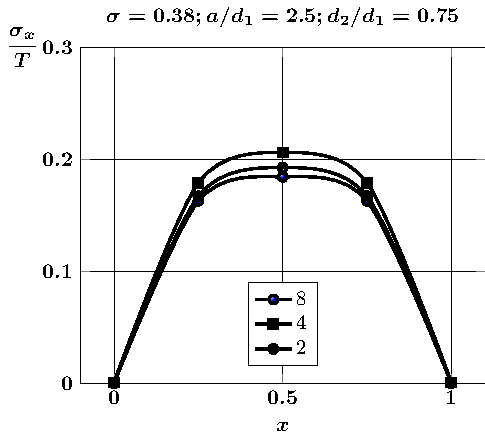
\includegraphics[width=7.5cm]{cav8-4-2-sig_x-spheroids.pdf}
\caption{Напряжения $\sigma_x/T$ на линии $AB$ в зависимости от количества полостей в тетрагональной структуре при одноосном растяжении пространства
\label{f:9:2}}}\hfil\hfil
\parbox[b]{7.5cm}{\centering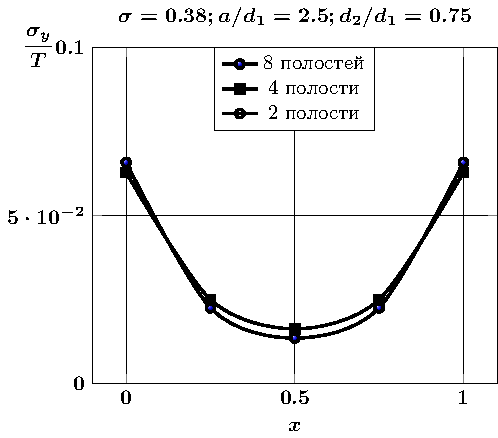
\includegraphics[width=7.5cm]{cav8-4-2-sig_y-spheroids.pdf}
\caption{Напряжения $\sigma_y/T$ на линии $AB$ в зависимости от количества полостей в тетрагональной структуре при одноосном растяжении пространства
\label{f:9:3}}}
\end{figure}

%\begin{figure}
%\centering
%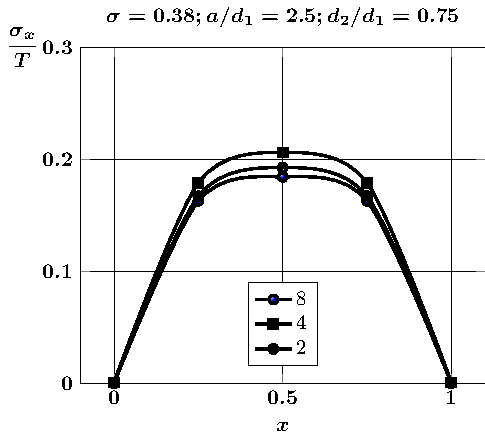
\includegraphics[width=11cm]{cav8-4-2-sig_x-spheroids.pdf}
%\caption{Напряжения $\sigma_x/T$ на линии $AB$ в зависимости от количества полостей в тетрагональной структуре при одноосном растяжении пространства}
%\label{f:9:2}
%\end{figure}
%
%\begin{figure}
%\centering
%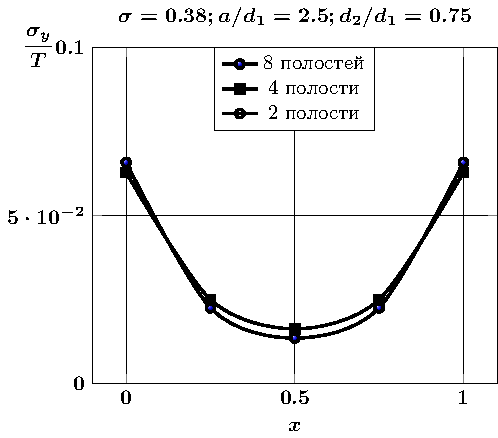
\includegraphics[width=11cm]{cav8-4-2-sig_y-spheroids.pdf}
%\caption{Напряжения $\sigma_y/T$ на линии $AB$ в зависимости от количества полостей в тетрагональной структуре при одноосном растяжении пространства}
%\label{f:9:3}
%\end{figure}

\begin{figure}[h!]
\centering\footnotesize
\parbox[b]{7.5cm}{\centering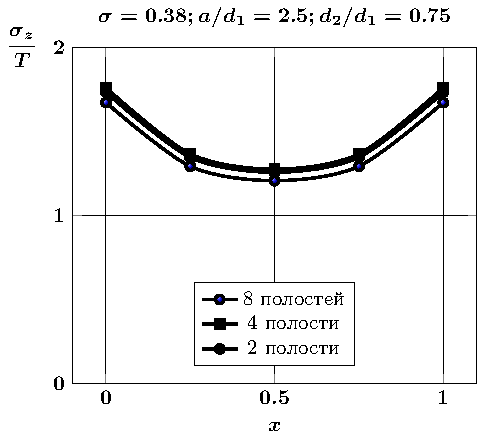
\includegraphics[width=7.5cm]{cav8-4-2-sig_z-spheroids.pdf}
\caption{Напряжения $\sigma_x/T$ на линии $AB$ для гексагональной и тетрагональной центрированных структур
\label{f:9:4}}}\hfil\hfil
\parbox[b]{7.5cm}{\centering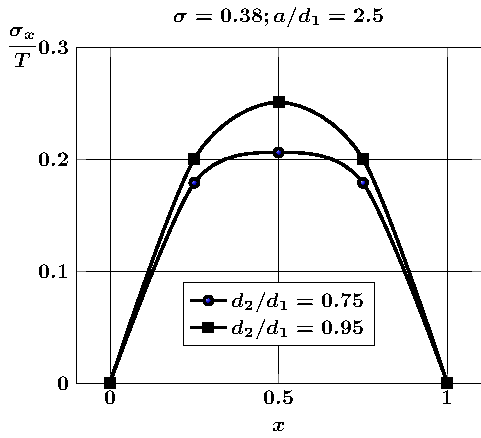
\includegraphics[width=7.5cm]{cav4-d-sig_x.pdf}
\caption{Напряжения $\sigma_x/T$ на линии $AB$ в зависимости от соотношения между полуосями сфероидов (четыре полости)
\label{f:9:5}}}
\end{figure}

%\begin{figure}
%\centering
%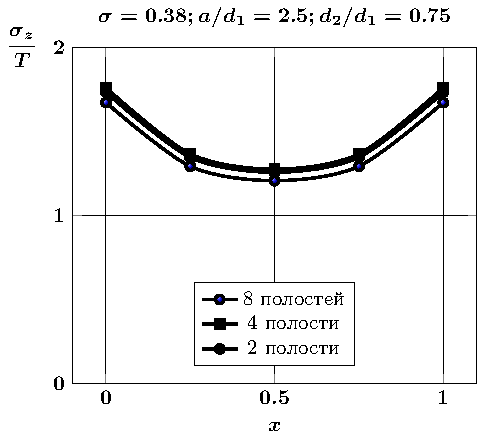
\includegraphics[width=11cm]{cav8-4-2-sig_z-spheroids.pdf}
%\caption{Напряжения $\sigma_z/T$ на линии $AB$ в зависимости от количества полостей в тетрагональной структуре при одноосном растяжении пространства}
%\label{f:9:4}
%\end{figure}
%
%\begin{figure}
%\centering
%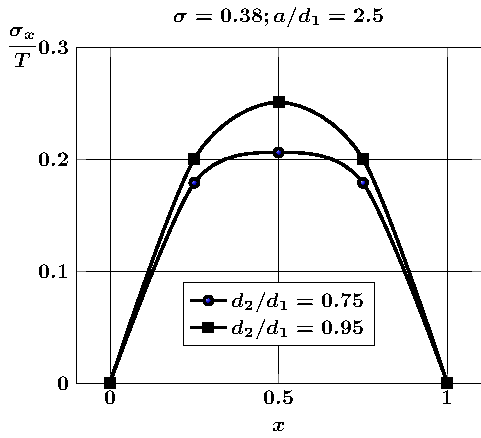
\includegraphics[width=12cm]{cav4-d-sig_x.pdf}
%\caption{Напряжения $\sigma_x/T$ на линии $AB$ в зависимости от соотношения между полуосями сфероидов (четыре полости)}
%\label{f:9:5}
%\end{figure}

\begin{figure}[h!]
\centering\footnotesize
\parbox[b]{7.5cm}{\centering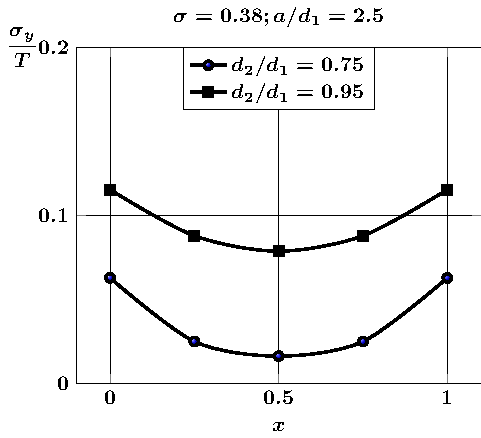
\includegraphics[width=7.5cm]{cav4-d-sig_y.pdf}
\caption{Напряжения $\sigma_y/T$ на линии $AB$ в зависимости от соотношения между полуосями сфероидов (четыре полости)
\label{f:9:6}}}\hfil\hfil
\parbox[b]{7.5cm}{\centering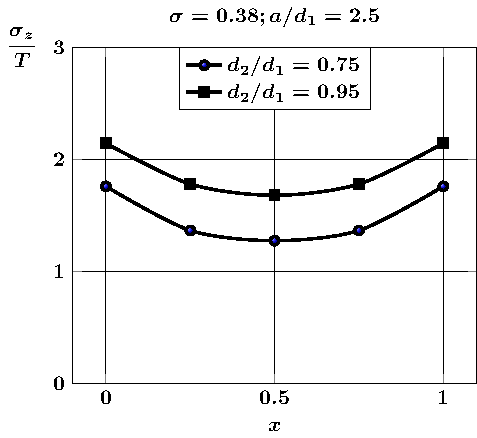
\includegraphics[width=7.5cm]{cav4-d-sig_z.pdf}
\caption{Напряжения $\sigma_z/T$ на линии $AB$ в зависимости соотношения между полуосями сфероидов (четыре полости)
\label{f:9:7}}}
\end{figure}

%\begin{figure}
%\centering
%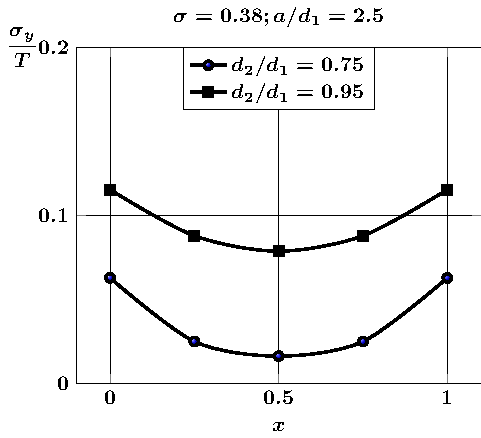
\includegraphics[width=12cm]{cav4-d-sig_y.pdf}
%\caption{Напряжения $\sigma_y/T$ на линии $AB$ в зависимости от соотношения между полуосями сфероидов (четыре полости)}
%\label{f:9:6}
%\end{figure}
%
%\begin{figure}
%\centering
%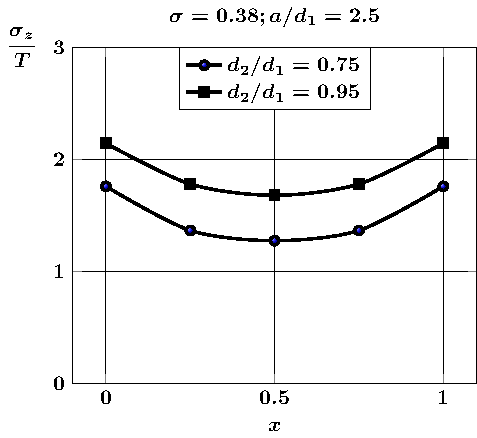
\includegraphics[width=12.2cm]{cav4-d-sig_z.pdf}
%\caption{Напряжения $\sigma_z/T$ на линии $AB$ в зависимости соотношения между полуосями сфероидов (четыре полости)}
%\label{f:9:7}
%\end{figure}

\begin{figure}[h!]
\centering\footnotesize
\parbox[b]{7.5cm}{\centering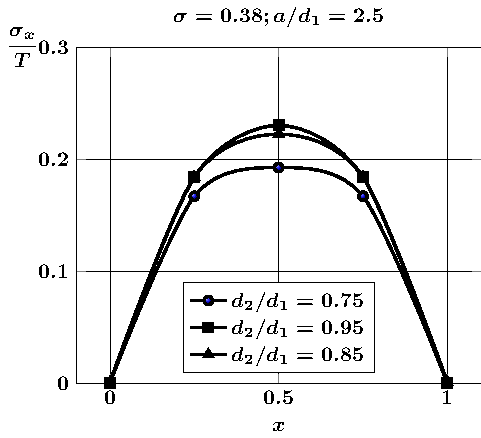
\includegraphics[width=7.5cm]{cav2-d-sig_x.pdf}
\caption{Напряжения $\sigma_x/T$ на линии $AB$ в зависимости от соотношения между полуосями сфероидов (две полости)
\label{f:9:8}}}\hfil\hfil
\parbox[b]{7.5cm}{\centering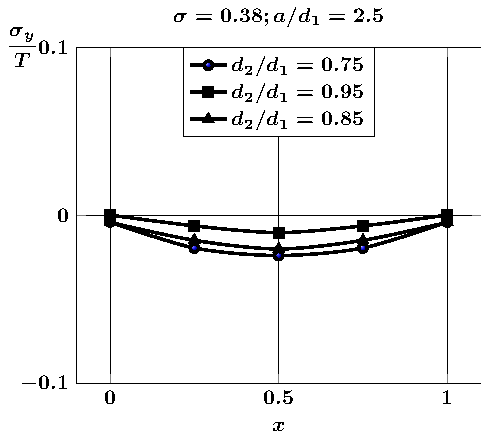
\includegraphics[width=7.5cm]{cav2-d-sig_y.pdf}
\caption{Напряжения $\sigma_y/T$ на линии $AB$ в зависимости от соотношения между полуосями сфероидов (две полости)
\label{f:9:9}}}
\end{figure}

%\begin{figure}
%\centering
%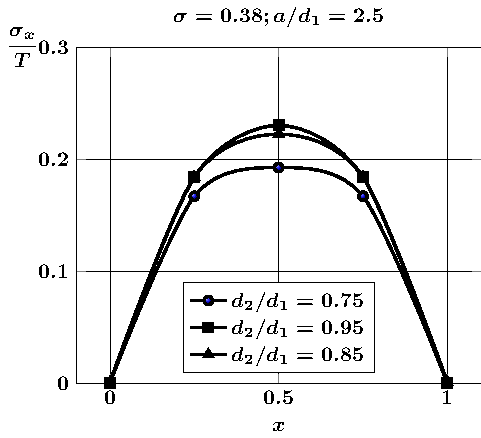
\includegraphics[width=12cm]{cav2-d-sig_x.pdf}
%\caption{Напряжения $\sigma_x/T$ на линии $AB$ в зависимости от соотношения между полуосями сфероидов (две полости)}
%\label{f:9:8}
%\end{figure}
%
%\begin{figure}
%\centering
%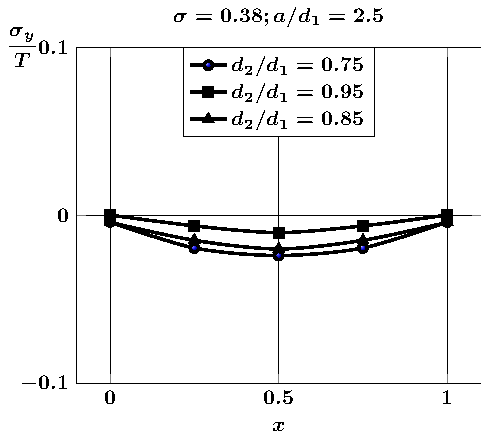
\includegraphics[width=12cm]{cav2-d-sig_y.pdf}
%\caption{Напряжения $\sigma_y/T$ на линии $AB$ в зависимости от соотношения между полуосями сфероидов (две полости)}
%\label{f:9:9}
%\end{figure}

Характерная особенность приведенных графиков заключается в том, что напряжения $\sigma_x/T$, $\sigma_y/T$ и $\sigma_z/T$ в средней точке отрезка с увеличением количества полостей сперва увеличиваются, а потом начинают убывать. Максимальные значения напряжений $\sigma_z/T$ на порядок выше максимальных зачений напряжений $\sigma_x/T$ и на два порядка~--- $\sigma_y/T$. Наблюдается характерная концентрация напряжений $\sigma_z/T$ на поверхностях полостей в их экваториальной плоскости. Максимальные напряжения $\sigma_z/T$ в 1.7 раза больше, чем растягивающие усилия на бесконечности.

На рис.~\ref{f:9:8}~--- \ref{f:9:10} приведены графики распределения напряжений $\sigma_x/T$, $\sigma_y/T$ и $\sigma_z/T$ вдоль горизонтальной  линии, соединяющей центры соседних сфероидальных полостей, в зависимости от соотношения полуосей сфероидов для двух полостей.

При увеличении отношения $d_2/d_1$ напряжения $\sigma_x/T$, $\sigma_z/T$ растут, а модуль напряжения $\sigma_y/T$ убывает.

Наблюдается существенное увеличение напряжений при сохранении общего характера в их распределении в случае увеличения отношения малой и большой полуосей сфероидов.

В табл.~\ref{t:9:1} приведены результаты данных проверки граничных условий на одной из сфероидальных полостей для конфигурации из пары полостей при одноосном растяжении и при $\sigma=0.38$, $a/d_1=2.5$, $d_1/d_2=0.75$, $n_{max}=6$, $p_{max}=r_{max}=10$.

В табл.~\ref{t:9:2} представлены результаты данных по сходимости метода редукции в средней точке линии, соединяющей центры пары сфероидальных полостей при одноосном растяжении и при $\sigma=0.38$, $a/d_1=2.5$, $d_1/d_2=0.75$.

\begin{figure}
\centering
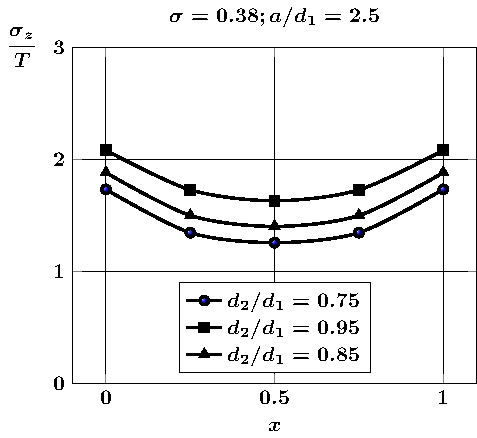
\includegraphics[width=8cm]{cav2-d-sig_z.pdf}
\caption{Напряжения $\sigma_z/T$ на линии $AB$ в зависимости соотношения между полуосями сфероидов (две полости)}
\label{f:9:10}
\end{figure}

Рассмотрим двуосное растяжение пространства с несколькими вытянутыми сфероидальными полостями. На рис.~\ref{f:9:11}~--- \ref{f:9:13} приведены графики распределения напряжений $\sigma_x/T$, $\sigma_y/T$ и $\sigma_z/T$ вдоль горизонтальной  линии, соединяющей центры соседних сфероидальных полостей, в зависимости от количества полостей в тетрагональной структуре для следующего набора параметров: $\sigma=0.38$, $a/d_1=2.5$, $d_2/d_1=0.75$.

На рис.~\ref{f:9:14}~--- \ref{f:9:29} представлены графики напряжений $\sigma_x/T$, $\sigma_y/T$ и $\sigma_z/T$ на линии $CD$ в тетрагональной структуре из сфероидальных полостей при одноосном и двуосном растяжениях пространства.

%\sidefig*(75mm){
%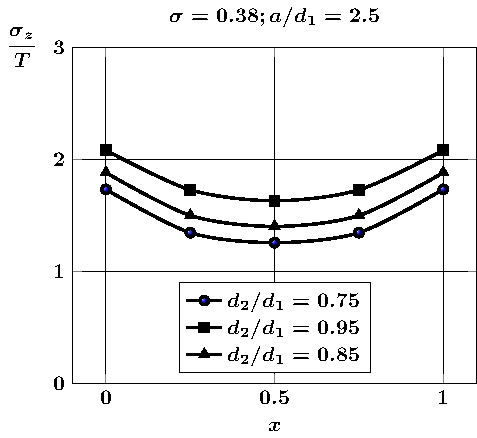
\includegraphics[width=7.5cm]{cav2-d-sig_z.pdf}
%\caption{Напряжения $\sigma_z/T$ на линии $AB$ в зависимости соотношения между полуосями сфероидов (две полости)}
%\label{f:9:10}
%}{Рассмотрим двуосное растяжение пространства с несколькими вытянутыми сфероидальными полостями. На рис.~\ref{f:9:11}~--- \ref{f:9:13} приведены графики распределения напряжений $\sigma_x/T$, $\sigma_y/T$ и $\sigma_z/T$ вдоль горизонтальной  линии, соединяющей центры соседних сфероидальных полостей, в зависимости от количества полостей в тетрагональной структуре для следующего набора параметров: $\sigma=0.38$, $a/d_1=2.5$, $d_2/d_1=0.75$.
%
%На рис.~\ref{f:9:14}~--- \ref{f:9:29} представлены графики напряжений $\sigma_x/T$, $\sigma_y/T$ и $\sigma_z/T$ на линии $CD$ в тетрагональной структуре из сфероидальных полостей при одноосном и двуосном растяжениях пространства.{\sloppy\par}
%}

\begin{table}[h]
\caption{Проверка граничных условий}
\centering
$
\begin{array}{|c|c|c|c|c|}
\hline
\eta & 0 & \dfrac{\pi}{2} & \pi & \dfrac{3\pi}{2} \\
\hline
\sigma_\rho & 0.000685503 & 1.44838\times 10^{-6} & 0.000356788 & 1.44838\times 10^{-6} \\
\hline
\end{array}
$
\label{t:9:1}
\end{table}

\begin{table}[h]
\caption{Сходимость метода редукции для сфероидальных полостей}
\centering
$
\begin{array}{|c|c|c|c|c|}
\hline
n_{max}; p_{max}; r_{max} & 5; 5; 5 & 6; 10; 10 & 8; 10; 10 & 10; 10; 10 \\
\hline
\sigma_x & 0.191411		& 0.192552 	& 0.19243 		& 0.19242 \\
\hline
\sigma_y & -0.0239008 	& -0.0239348 	& -0.0239318 	& -0.0239316 \\
\hline
\sigma_z & 1.25566 		& 1.25552 		& 1.25556 		& 1.25557 \\
\hline
\end{array}
$
\label{t:9:2}
\end{table}

%\begin{figure}
%\centering
%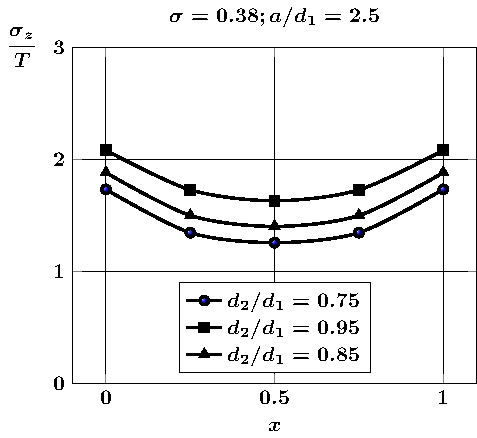
\includegraphics[width=12cm]{cav2-d-sig_z.pdf}
%\caption{Напряжения $\sigma_z/T$ на линии $AB$ в зависимости соотношения между полуосями сфероидов (две полости)}
%\label{f:9:10}
%\end{figure}

%\subsection{Анализ численных результатов для пространства с вытянутыми сфероидальными полостями при двуосном растяжении}

\begin{figure}[h!]
\centering\footnotesize
\parbox[b]{7.5cm}{\centering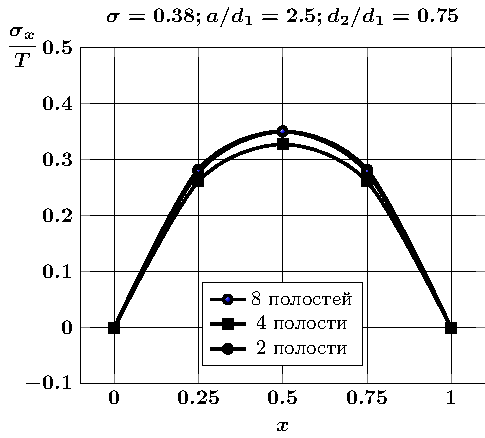
\includegraphics[width=7.5cm]{cav8-4-2-sig_x-spheroids-tension2.pdf}
\caption{Напряжения $\sigma_x/T$ на линии $AB$ в зависимости от количества полостей в тетрагональной структуре при двуосном растяжении пространства
\label{f:9:11}}}\hfil\hfil
\parbox[b]{7.5cm}{\centering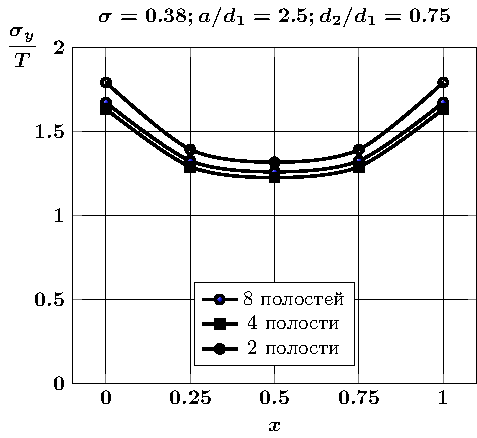
\includegraphics[width=7.5cm]{cav8-4-2-sig_y-spheroids-tension2.pdf}
\caption{Напряжения $\sigma_y/T$ на линии $AB$ в зависимости от количества полостей в тетрагональной структуре при двуосном растяжении пространства
\label{f:9:12}}}
\end{figure}

%\begin{figure}
%\centering
%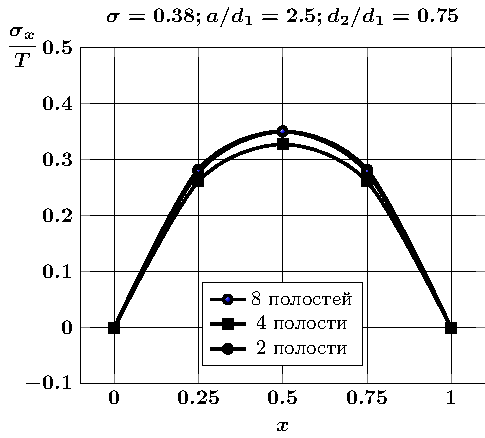
\includegraphics[width=11cm]{cav8-4-2-sig_x-spheroids-tension2.pdf}
%\caption{Напряжения $\sigma_x/T$ на линии $AB$ в зависимости от количества полостей в тетрагональной структуре при двуосном растяжении пространства}
%\label{f:9:11}
%\end{figure}
%
%\begin{figure}
%\centering
%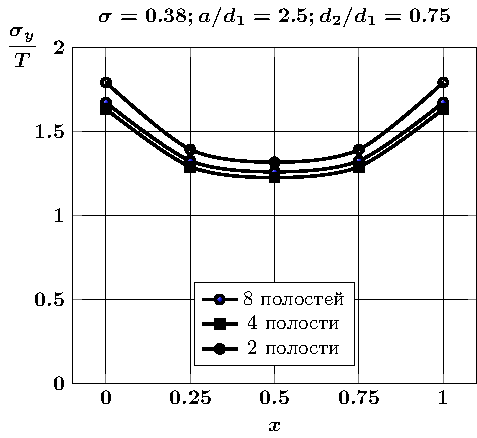
\includegraphics[width=11cm]{cav8-4-2-sig_y-spheroids-tension2.pdf}
%\caption{Напряжения $\sigma_y/T$ на линии $AB$ в зависимости от количества полостей в тетрагональной структуре при двуосном растяжении пространства}
%\label{f:9:12}
%\end{figure}

\begin{figure}[h!]
\centering\footnotesize
\parbox[b]{7.5cm}{\centering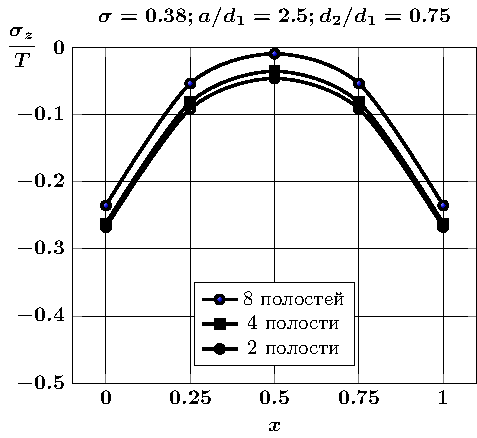
\includegraphics[width=7.5cm]{cav8-4-2-sig_z-spheroids-tension2.pdf}
\caption{Напряжения $\sigma_z/T$ на линии $AB$ в зависимости от количества полостей в тетрагональной структуре при двуосном растяжении пространства
\label{f:9:13}}}\hfil\hfil
\parbox[b]{7.5cm}{\centering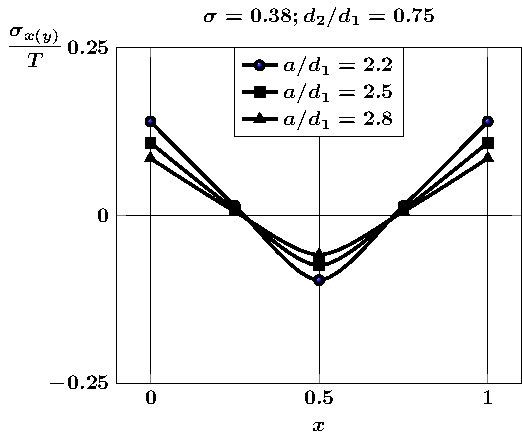
\includegraphics[width=8cm]{cav8-a-d75-t1-sig_x-cd.pdf}
\caption{Напряжения $\sigma_x/T$, $\sigma_y/T$ на линии $CD$ в тетрагональной структуре из сфероидальных полостей в зависимости от расстояния между полостями при одноосном растяжении пространства
\label{f:9:14}}}
\end{figure}

%\begin{figure}
%\centering
%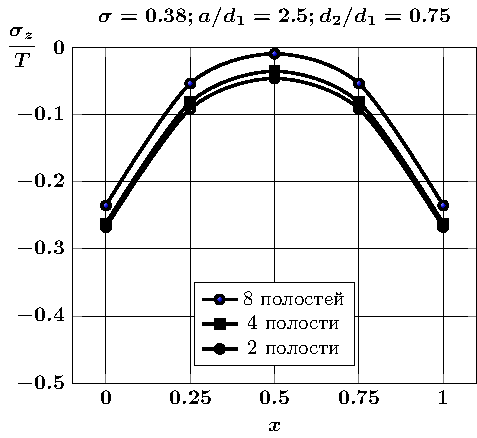
\includegraphics[width=11cm]{cav8-4-2-sig_z-spheroids-tension2.pdf}
%\caption{Напряжения $\sigma_z/T$ на линии $AB$ в зависимости от количества полостей в тетрагональной структуре при двуосном растяжении пространства}
%\label{f:9:13}
%\end{figure}
%
%\begin{figure}
%\centering
%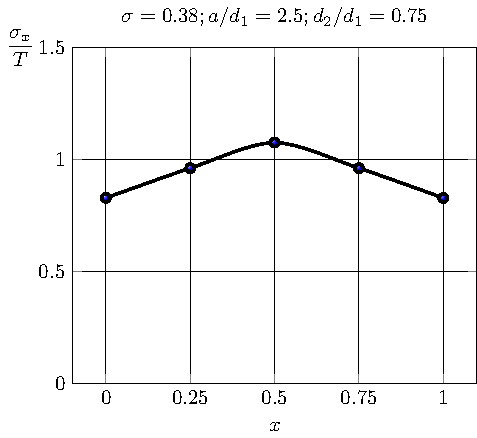
\includegraphics[width=11cm]{cav8-a25-c-c-sig_x-spheroids-tension2.pdf}
%\caption{Напряжения $\sigma_x/T$ на линии $CD$ в тетрагональной структуре из сфероидальных полостей при двуосном растяжении пространства}
%\label{f:9:14}
%\end{figure}

\begin{figure}[h!]
\centering\footnotesize
\parbox[b]{7.5cm}{\centering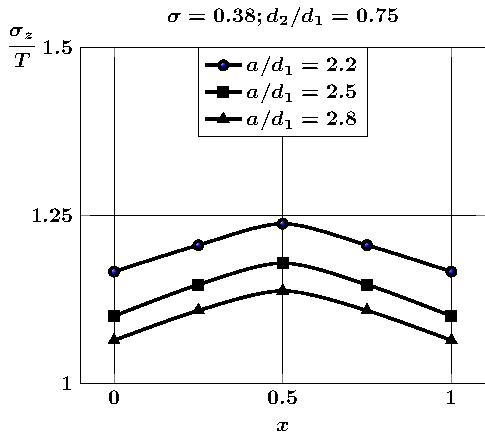
\includegraphics[width=7.5cm]{cav8-a-d75-t1-sig_z-cd.pdf}
\caption{Напряжения $\sigma_z/T$ на линии $CD$ в тетрагональной структуре из сфероидальных полостей в зависимости от расстояния между полостями при одноосном растяжении пространства
\label{f:9:15}}}\hfil\hfil
\parbox[b]{7.5cm}{\centering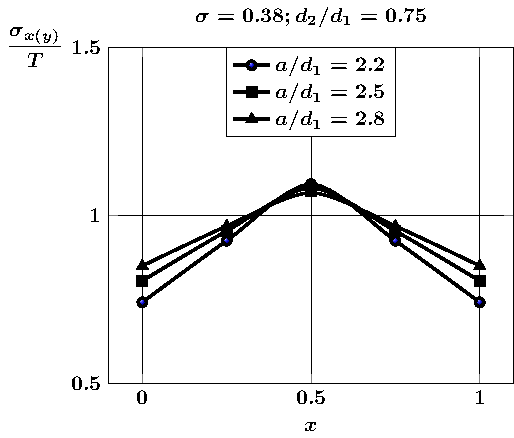
\includegraphics[width=8cm]{cav8-a-d75-t2-sig_x-cd.pdf}
\caption{Напряжения $\sigma_x/T$ на линии $CD$ в тетрагональной структуре из сфероидальных полостей в зависимости от расстояния между полостями при двуосном растяжении пространства
\label{f:9:16}}}
\end{figure}

\begin{figure}[h!]
\centering\footnotesize
\parbox[b]{7.5cm}{\centering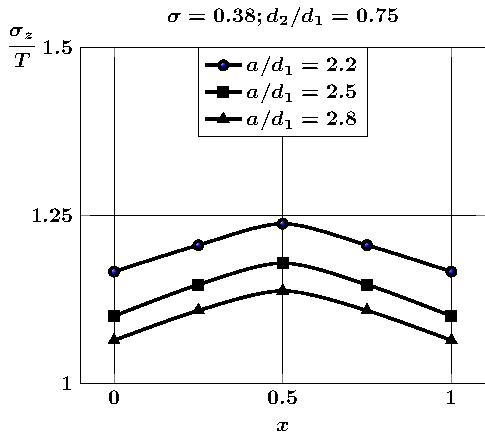
\includegraphics[width=7.5cm]{cav8-a-d75-t1-sig_z-cd.pdf}
\caption{Напряжения $\sigma_z/T$ на линии $CD$ в тетрагональной структуре из сфероидальных полостей в зависимости от расстояния между полостями при двуосном растяжении пространства
\label{f:9:29}}}\hfil\hfil
\parbox[b]{7.5cm}{\centering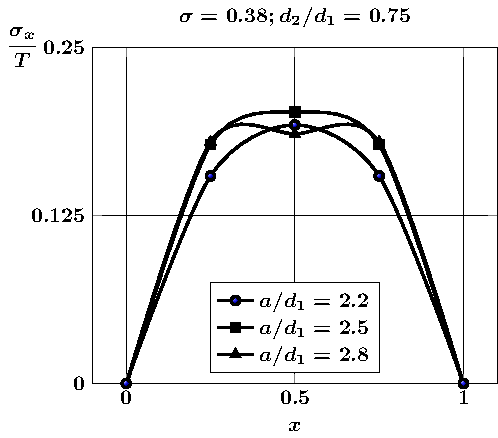
\includegraphics[width=7.5cm]{cav8-a-d75-t1-sig_x-ab.pdf}
\caption{Напряжения $\sigma_x/T$ на линии $AB$ в тетрагональной структуре из сфероидальных полостей в зависимости от расстояния между полостями при одноосном растяжении пространства
\label{f:9:30}}}
\end{figure}

%\begin{figure}
%\centering
%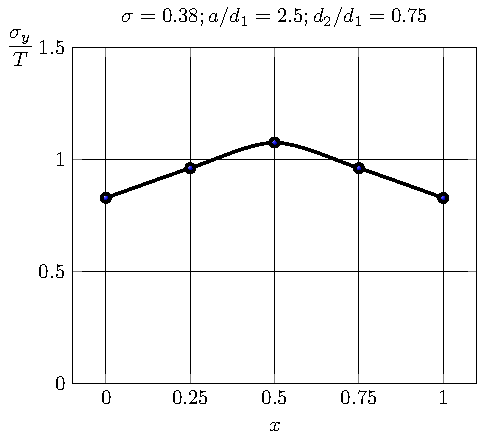
\includegraphics[width=11cm]{cav8-a25-c-c-sig_y-spheroids-tension2.pdf}
%\caption{Напряжения $\sigma_y/T$ на линии $CD$ в тетрагональной структуре из сфероидальных полостей при двуосном растяжении пространства}
%\label{f:9:15}
%\end{figure}
%
%\begin{figure}
%\centering
%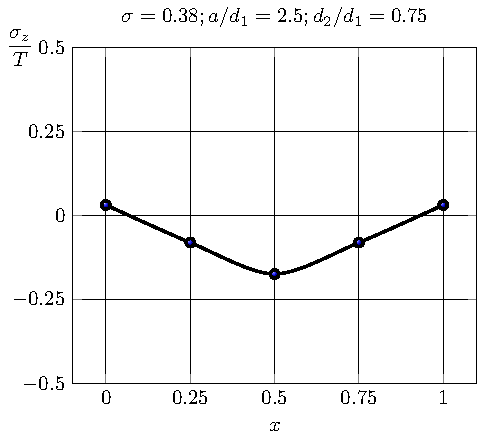
\includegraphics[width=11cm]{cav8-a25-c-c-sig_z-spheroids-tension2.pdf}
%\caption{Напряжения $\sigma_z/T$ на линии $CD$ в тетрагональной структуре из сфероидальных полостей при двуосном растяжении пространства}
%\label{f:9:16}
%\end{figure}

Наблюдается практически линейный характер распределения напряжений между средней точкой отрезка $CD$ и любым из его концов. Для напряжений $\sigma_x/T$, $\sigma_y/T$ имеются области растягивающих напряжений в окрестности оснований кубической ячейки. Напряжения   $\sigma_z/T$ растут при приближении полостей друг к другу.

\begin{figure}[h!]
\centering\footnotesize
\parbox[b]{7.5cm}{\centering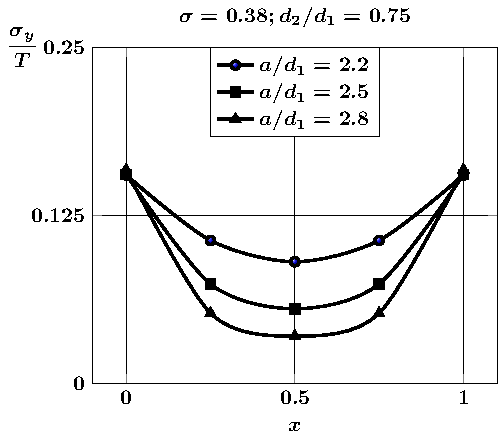
\includegraphics[width=8.2cm]{cav8-a-d75-t1-sig_y-ab.pdf}
\caption{Напряжения $\sigma_y/T$ на линии $AB$ в тетрагональной структуре из сфероидальных полостей в зависимости от расстояния между полостями при одноосном растяжении пространства
\label{f:9:31}}}\hfil\hfil
\parbox[b]{7.5cm}{\centering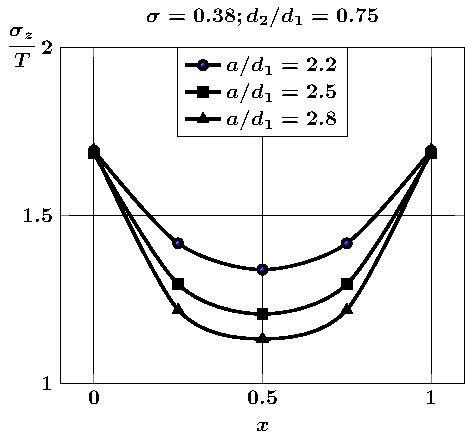
\includegraphics[width=7.8cm]{cav8-a-d75-t1-sig_z-ab.pdf}
\caption{Напряжения $\sigma_z/T$ на линии $AB$ в тетрагональной структуре из сфероидальных полостей в зависимости от расстояния между полостями при одноосном растяжении пространства
\label{f:9:32}}}
\end{figure}

\begin{figure}[h!]
\centering\footnotesize
\parbox[b]{7.5cm}{\centering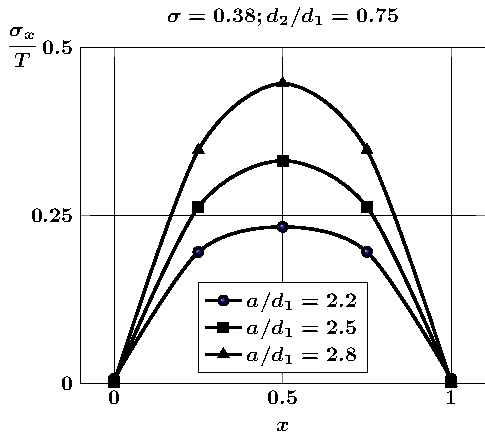
\includegraphics[width=8cm]{cav8-a-d75-t2-sig_x-ab.pdf}
\caption{Напряжения $\sigma_x/T$ на линии $AB$ в тетрагональной структуре из сфероидальных полостей в зависимости от расстояния между полостями при двуосном растяжении пространства
\label{f:9:33}}}\hfil\hfil
\parbox[b]{7.5cm}{\centering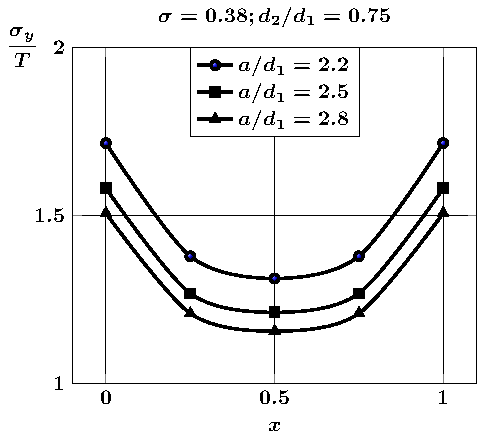
\includegraphics[width=8cm]{cav8-a-d75-t2-sig_y-ab.pdf}
\caption{Напряжения $\sigma_y/T$ на линии $AB$ в тетрагональной структуре из сфероидальных полостей в зависимости от расстояния между полостями при двуосном растяжении пространства
\label{f:9:34}}}
\end{figure}

Для двуосного растяжения характер распределения напряжений $\sigma_x/T$, $\sigma_y/T$, $\sigma_z/T$ напоминает случай одноосного растяжения, только с заменой $\sigma_x/T$, $\sigma_y/T$ на $\sigma_z/T$.

На рис.~\ref{f:9:30}~--- \ref{f:9:32} приведены напряжения $\sigma_x/T$, $\sigma_y/T$, $\sigma_z/T$ на линии $AB$ при одноосном растяжении в зависимости от относительного расстояния $a/d_1$ между полостями.

Основной вклад в тензор напряжений вносят напряжения $\sigma_z/T$. Областью концентрации напряжений $\sigma_y/T$, $\sigma_z/T$ является граница полостей, в то время как напряжения $\sigma_x/T$ достигают максимальных значений в средней точке отрезка $AB$. Напряжения $\sigma_y/T$, $\sigma_z/T$ растут с приближением полостей друг к другу.

\begin{figure}[h!]
\centering
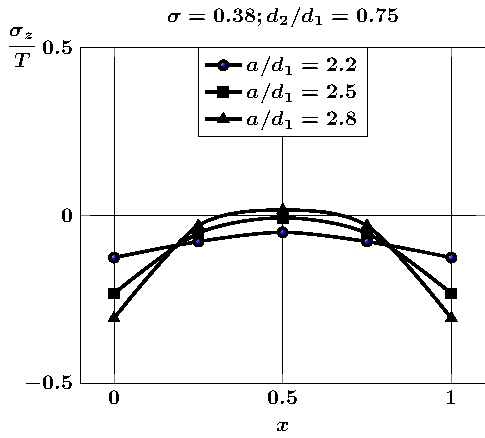
\includegraphics[width=8cm]{cav8-a-d75-t2-sig_z-ab.pdf}
\caption{Напряжения $\sigma_z/T$ на линии $AB$ в тетрагональной структуре из сфероидальных полостей в зависимости от расстояния между полостями при двуосном растяжении пространства}
\label{f:9:35}
\end{figure}

На рис.~\ref{f:9:33}~--- \ref{f:9:35} приведены напряжения $\sigma_x/T$, $\sigma_y/T$, $\sigma_z/T$ на линии $AB$ при двуосном растяжении в зависимости от относительного расстояния $a/d_1$ между полостями.

Основной вклад в тензор напряжений вносят напряжения $\sigma_y/T$. Областью их концентрации являются границы полостей. Напряжения $\sigma_x/T$ убывают, а $\sigma_y/T$ растут при приближении полостей друг к другу. Напряжения $\sigma_z/T$ с приближением полостей друг к другу стремятся к сжимающим постоянным напряжениям.

%\sidefig*(85mm){
%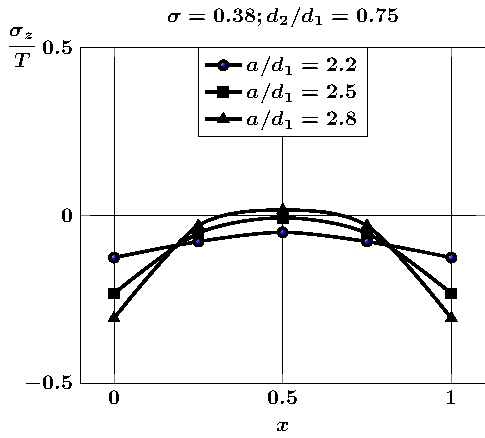
\includegraphics[width=8cm]{cav8-a-d75-t2-sig_z-ab.pdf}
%\caption{Напряжения $\sigma_z/T$ на линии $AB$ в тетрагональной структуре из сфероидальных полостей в зависимости от расстояния между полостями при двуосном растяжении пространства}
%\label{f:9:35}
%}{
%На рис.~\ref{f:9:33}~--- \ref{f:9:35} приведены напряжения $\sigma_x/T$, $\sigma_y/T$, $\sigma_z/T$ на линии $AB$ при двуосном растяжении в зависимости от относительного расстояния $a/d_1$ между полостями.
%
%Основной вклад в тензор напряжений вносят напряжения $\sigma_y/T$. Областью их концентрации являются границы полостей. Напряжения $\sigma_x/T$ убывают, а $\sigma_y/T$ растут при приближении полостей друг к другу. Напряжения $\sigma_z/T$ с приближением полостей друг к другу стремятся к сжимающим постоянным напряжениям.
%}

\subsection{Тетрагональная центрированная структура расположения сфероидальных полостей в материале}

Рассмотрим тетрагональную центрированную структуру расположения сфероидальных полостей в пористом материале (см.~рис.~\ref{f:9:42}).

\begin{figure}[h!]
\centering
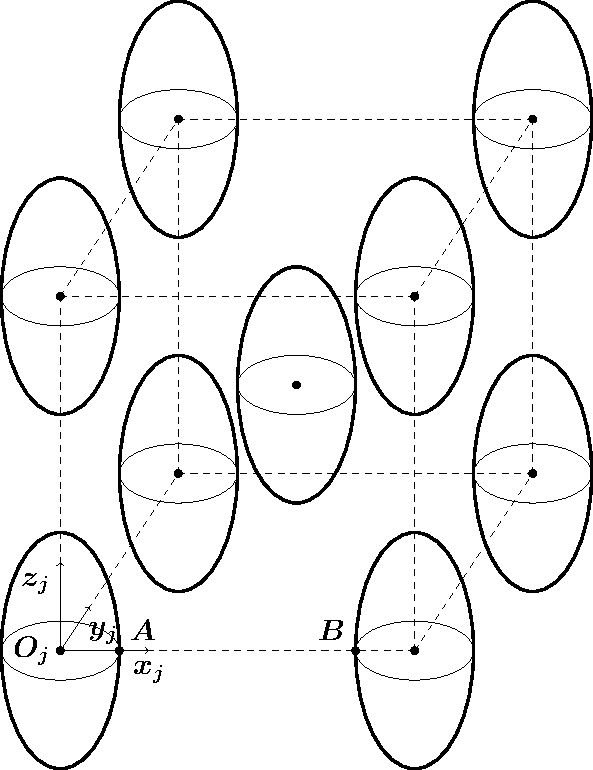
\includegraphics[width=6cm]{cav-9.pdf}
\caption{Одна ячейка тетрагональной центрированной структуры}
\label{f:9:42}
\end{figure}

\begin{figure}[h!]
\centering\footnotesize
\parbox[b]{7.5cm}{\centering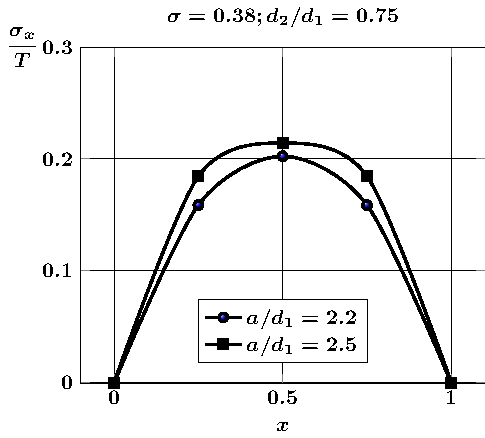
\includegraphics[width=7.5cm]{cav9-a-d75-t1-sig_x.pdf}
\caption{Напряжения $\sigma_x/T$ на линии $AB$ в тетрагональной центрированной структуре в зависимости от расстояния между полостями при одноосном растяжении 
\label{f:9:36}}}\hfil\hfil
\parbox[b]{7.5cm}{\centering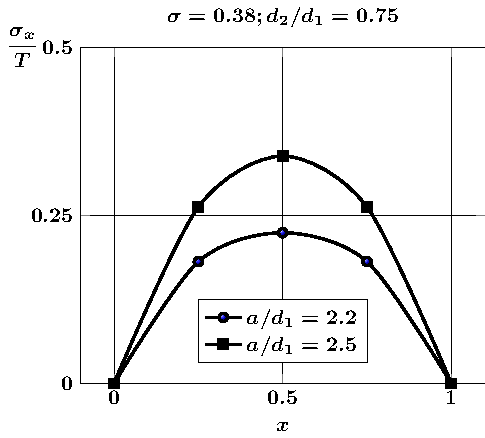
\includegraphics[width=7.5cm]{cav9-a-d75-t2-sig_x.pdf}
\caption{Напряжения $\sigma_x/T$ на линии $AB$ в тетрагональной центрированной структуре в зависимости от расстояния между полостями при двуосном растяжении
\label{f:9:37}}}
\end{figure}

На рис.~\ref{f:9:36}~--- \ref{f:9:41} приведены графики напряжений $\sigma_x/T$, $\sigma_y/T$ и $\sigma_z/T$ для одной ячейки тетрагональной центрированной структуры на линии $AB$ в зависимости от относительного расстояния $a/d_1$ между полостями при одноосном и двуосном растяжениях упругого пространства при $d_2/d_1=0.75$, $\sigma=0.38$.

\begin{figure}[h!]
\centering\footnotesize
\parbox[b]{7.5cm}{\centering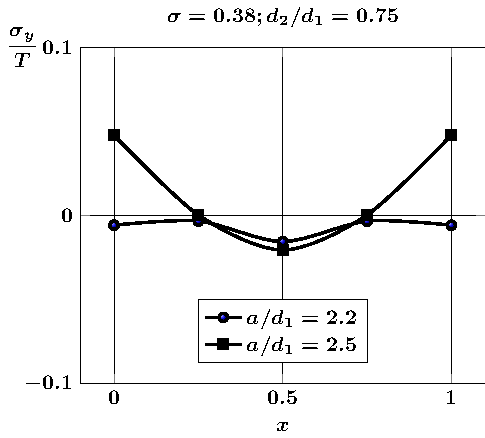
\includegraphics[width=7.5cm]{cav9-a-d75-t1-sig_y.pdf}
\caption{Напряжения $\sigma_y/T$ на линии $AB$ в тетрагональной центрированной структуре в зависимости от расстояния между полостями при одноосном растяжении 
\label{f:9:38}}}\hfil\hfil
\parbox[b]{7.5cm}{\centering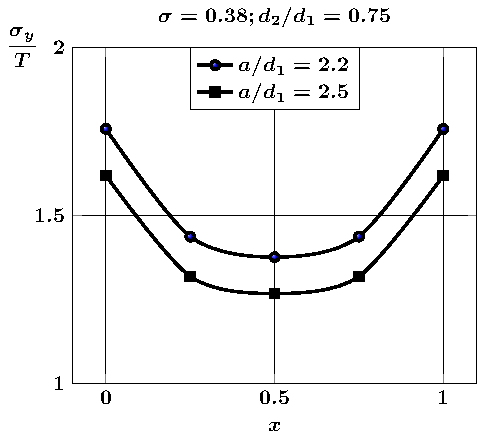
\includegraphics[width=7.5cm]{cav9-a-d75-t2-sig_y.pdf}
\caption{Напряжения $\sigma_y/T$ на линии $AB$ в тетрагональной центрированной структуре в зависимости от расстояния между полостями при двуосном растяжении
\label{f:9:39}}}
\end{figure}

\begin{figure}[h!]
\centering\footnotesize
\parbox[b]{7.5cm}{\centering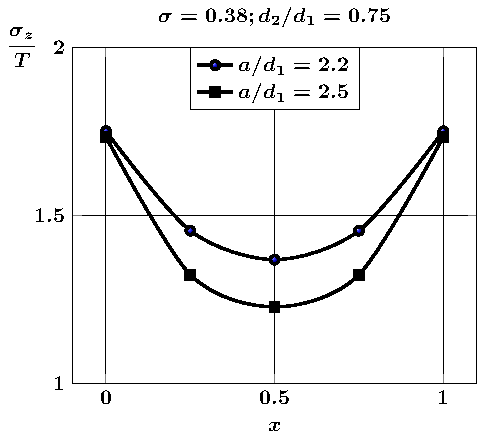
\includegraphics[width=7.5cm]{cav9-a-d75-t1-sig_z.pdf}
\caption{Напряжения $\sigma_z/T$ на линии $AB$ в тетрагональной центрированной структуре в зависимости от расстояния между полостями при одноосном растяжении 
\label{f:9:40}}}\hfil\hfil
\parbox[b]{7.5cm}{\centering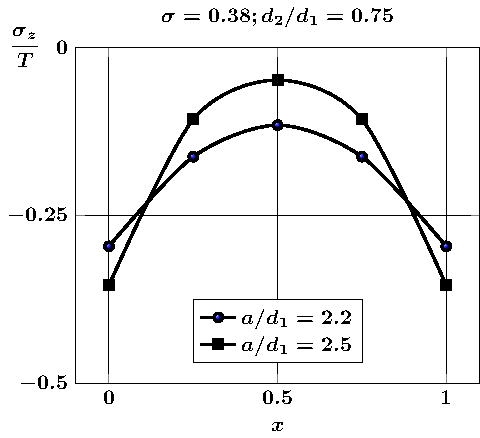
\includegraphics[width=7.5cm]{cav9-a-d75-t2-sig_z.pdf}
\caption{Напряжения $\sigma_z/T$ на линии $AB$ в тетрагональной центрированной структуре в зависимости от расстояния между полостями при двуосном растяжении
\label{f:9:41}}}
\end{figure}

При одноосном растяжении основной вклад в тензор напряжений вносят напряжения $\sigma_z/T$. Областью их концентрации являются границы полостей, и они растут с приближением полостей друг к другу. При двуосном растяжении подобными свойствами обладают напряжения $\sigma_y/T$. Напряжения $\sigma_z/T$ являются сжимающими на всем отрезке $AB$.

\subsection{Гексагональная центрированная структура расположения сфероидальных полостей в материале}

Рассмотрим гексагональную центрированную структуру расположения сфероидальных полостей в пористом материале (см.~рис.~\ref{f:9:43}).

\begin{figure}[h!]
\centering
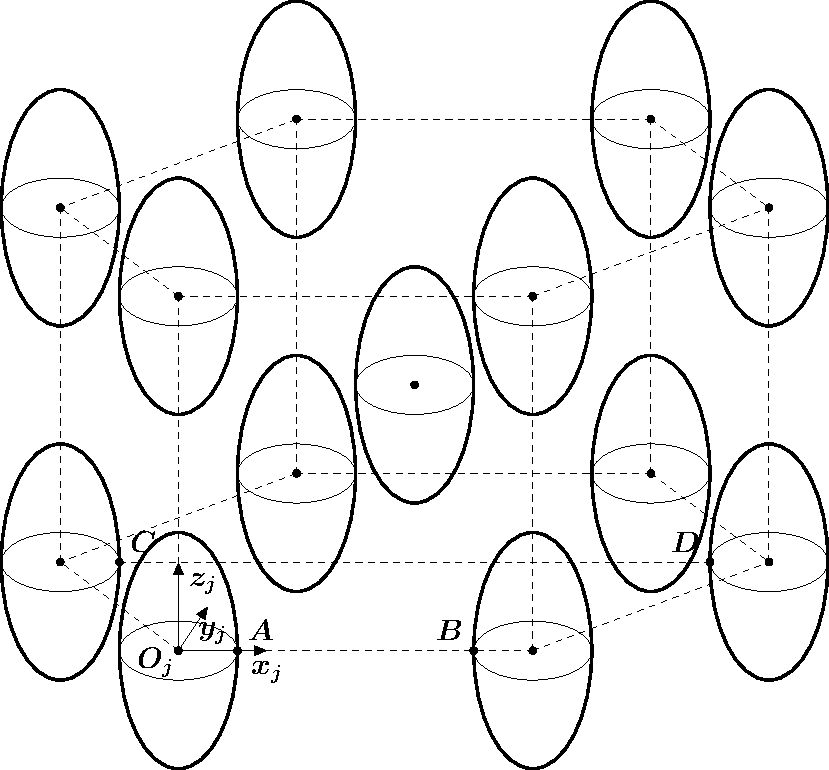
\includegraphics[width=7cm]{cav-13.pdf}
\caption{Одна ячейка гексагональной центрированной структуры}
\label{f:9:43}
\end{figure}

\begin{figure}[h!]
\centering\footnotesize
\parbox[b]{7.5cm}{\centering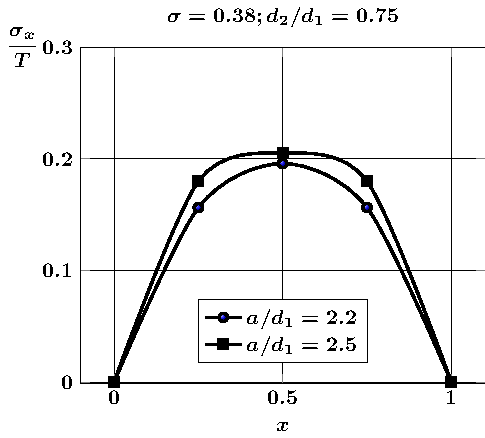
\includegraphics[width=7.5cm]{cav13-a-d75-t1-sig_x.pdf}
\caption{Напряжения $\sigma_x/T$ на линии $AB$ в гексагональной центрированной структуре в зависимости от расстояния между полостями при одноосном растяжении 
\label{f:9:44}}}\hfil\hfil
\parbox[b]{7.5cm}{\centering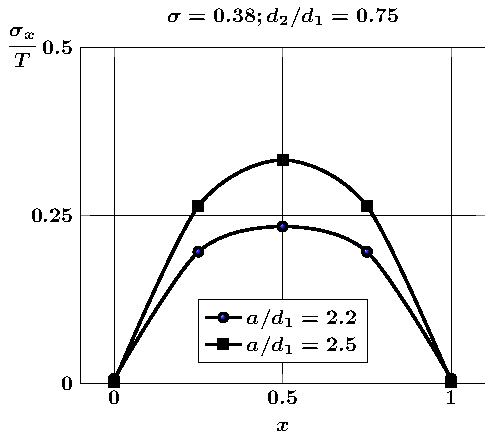
\includegraphics[width=7.5cm]{cav13-a-d75-t2-sig_x.pdf}
\caption{Напряжения $\sigma_x/T$ на линии $AB$ в гексагональной центрированной структуре в зависимости от расстояния между полостями при двуосном растяжении
\label{f:9:45}}}
\end{figure}

На рис.~\ref{f:9:44}~--- \ref{f:9:49} приведены графики напряжений $\sigma_x/T$, $\sigma_y/T$ и $\sigma_z/T$ для одной ячейки гексагональной центрированной структуры на линии $AB$ в зависимости от относительного расстояния $a/d_1$ между полостями при одноосном и двуосном растяжении упругого пространства при $d_2/d_1=0.75$, $\sigma=0.38$.

\begin{figure}[h!]
\centering\footnotesize
\parbox[b]{7.5cm}{\centering\includegraphics[width=7.5cm]{cav13-a-d75-t1-sig_y.pdf}
\caption{Напряжения $\sigma_y/T$ на линии $AB$ в гексагональной центрированной структуре в зависимости от расстояния между полостями при одноосном растяжении 
\label{f:9:46}}}\hfil\hfil
\parbox[b]{7.5cm}{\centering\includegraphics[width=7.5cm]{cav13-a-d75-t2-sig_y.pdf}
\caption{Напряжения $\sigma_y/T$ на линии $AB$ в гексагональной центрированной структуре в зависимости от расстояния между полостями при двуосном растяжении
\label{f:9:47}}}
\end{figure}

\begin{figure}[h!]
\centering\footnotesize
\parbox[b]{7.5cm}{\centering\includegraphics[width=7.5cm]{cav13-a-d75-t1-sig_z.pdf}
\caption{Напряжения $\sigma_z/T$ на линии $AB$ в гексагональной центрированной структуре в зависимости от расстояния между полостями при одноосном растяжении 
\label{f:9:48}}}\hfil\hfil
\parbox[b]{7.5cm}{\centering\includegraphics[width=7.5cm]{cav13-a-d75-t2-sig_z.pdf}
\caption{Напряжения $\sigma_z/T$ на линии $AB$ в гексагональной центрированной структуре в зависимости от расстояния между полостями при двуосном растяжении
\label{f:9:49}}}
\end{figure}

При одноосном растяжении основной вклад в тензор напряжений вносят напряжения $\sigma_z/T$. Областью их концентрации являются границы полостей, и они растут с приближением полостей друг к другу. При двуосном растяжении подобными свойствами обладают напряжения $\sigma_y/T$. Напряжения $\sigma_z/T$ являются сжимающими на всем отрезке $AB$.

\begin{figure}[h!]
\centering\footnotesize
\parbox[b]{7.5cm}{\centering\includegraphics[width=7.5cm]{cav13-a-d75-t1-sig_x-cd.pdf}
\caption{Напряжения $\sigma_x/T$ на линии $CD$ в гексагональной центрированной структуре в зависимости от расстояния между полостями при одноосном растяжении 
\label{f:9:50}}}\hfil\hfil
\parbox[b]{7.5cm}{\centering\includegraphics[width=7.5cm]{cav13-a-d75-t2-sig_x-cd.pdf}
\caption{Напряжения $\sigma_x/T$ на линии $CD$ в гексагональной центрированной структуре в зависимости от расстояния между полостями при двуосном растяжении
\label{f:9:51}}}
\end{figure}

\begin{figure}[h!]
\centering\footnotesize
\parbox[b]{7.5cm}{\centering\includegraphics[width=7.5cm]{cav13-a-d75-t1-sig_y-cd.pdf}
\caption{Напряжения $\sigma_y/T$ на линии $CD$ в гексагональной центрированной структуре в зависимости от расстояния между полостями при одноосном растяжении 
\label{f:9:52}}}\hfil\hfil
\parbox[b]{7.5cm}{\centering\includegraphics[width=7.5cm]{cav13-a-d75-t2-sig_y-cd.pdf}
\caption{Напряжения $\sigma_y/T$ на линии $CD$ в гексагональной центрированной структуре в зависимости от расстояния между полостями при двуосном растяжении
\label{f:9:53}}}
\end{figure}

На рис.~\ref{f:9:50}~--- \ref{f:9:55} приведены графики напряжений $\sigma_x/T$, $\sigma_y/T$ и $\sigma_z/T$ для одной ячейки гексагональной центрированной структуры на линии $CD$ в зависимости от относительного расстояния $a/d_1$ между полостями при одноосном и двуосном растяжениях упругого пространства при $d_2/d_1=0.75$, $\sigma=0.38$.

\begin{figure}[h!]
\centering\footnotesize
\parbox[b]{7cm}{\centering\includegraphics[width=7cm]{cav13-a-d75-t1-sig_z-cd.pdf}
\caption{Напряжения $\sigma_z/T$ на линии $CD$ в гексагональной центрированной структуре в зависимости от расстояния между полостями при одноосном растяжении 
\label{f:9:54}}}\hfil\hfil
\parbox[b]{7cm}{\centering\includegraphics[width=7cm]{cav13-a-d75-t2-sig_z-cd.pdf}
\caption{Напряжения $\sigma_z/T$ на линии $CD$ в гексагональной центрированной структуре в зависимости от расстояния между полостями при двуосном растяжении
\label{f:9:55}}}
\end{figure}

\begin{figure}[h!]
\centering\footnotesize
\parbox[b]{7.5cm}{\centering\includegraphics[width=7.6cm]{cav13-9-a25-t1.pdf}
\caption{Сравнение напряжений на линии $AB$ для одной ячейки центрированных тетрагональной и гексагональной структур при одноосном растяжении 
\label{f:9:56}}}\hfil\hfil
\parbox[b]{7.5cm}{\centering\includegraphics[width=7.6cm]{cav13-9-a25-t2.pdf}
\caption{Сравнение напряжений на линии $AB$ для одной ячейки центрированных тетрагональной и гексагональной структур при двуосном растяжении
\label{f:9:57}}}
\end{figure}

В случае одноосного растяжения основной вклад в тензор напряжений вносят напряжения $\sigma_z/T$. Областью их концентрации являются границы полостей. В середине отрезка $CD$ напряжения $\sigma_z/T$ близки к нулю. Зависимость напряжений от расстояния между полостями несущественна.

При двуосном растяжении главный вклад в тензор напряжений вносят напряжения $\sigma_x/T$ и $\sigma_y/T$, которые в средней точке отрезка $CD$ достигают максимального значения и совпадают. Напряжения $\sigma_z/T$ меняют знак на рассматриваемом отрезке, оставаясь сжимающими вблизи границ полостей и растягивающими в средней части отрезка $CD$.

На рис.~\ref{f:9:56}, \ref{f:9:57} приведено сравнение нормальных напряжений для одной ячейки центрированных тетрагональной и гексагональной структур на отрезке $AB$ при одноосном и двуосном растяжении упругого пространства. Графики показывают, что распределения напряжений для указанных структур практически не отличаются.

\begin{figure}[h!]
\centering\footnotesize
\parbox[b]{7.5cm}{\centering\includegraphics[width=7.6cm]{cav13-d-a25-t1.pdf}
\caption{Сравнение напряжений на линии $AB$ для одной ячейки центрированной гексагональной структуры в зависимости от формы полостей при одноосном растяжении 
\label{f:9:58}}}\hfil\hfil
\parbox[b]{7.5cm}{\centering\includegraphics[width=7.6cm]{cav13-d-a25-t2.pdf}
\caption{Сравнение напряжений на линии $AB$ для одной ячейки центрированной гексагональной структуры в зависимости от формы полостей при двуосном растяжении
\label{f:9:59}}}
\end{figure}

На рис.~\ref{f:9:58}, \ref{f:9:59} представлено сравнение напряжений на линии $AB$ для одной ячейки центрированной гексагональной структуры в зависимости от формы полостей при одноосном и двуосном растяжениях упругого пространства. При одноосном растяжении наибольшее отличие наблюдается при сравнении напряжений $\sigma_y/T$ и $\sigma_z/T$, причем полостям с меньшей кривизной соответствуют большие значения напряжений. В двуосном случае в отличие от одноосного заметна разница в распределении напряжений $\sigma_x/T$.

\section[Упругое состояние пространства с несколькими вытянутыми сфероидальными включениями]{Упругое состояние пространства с несколькими вытянутыми сфероидальными включениями\sectionmark{Упругое состояние пространства со сфероидальными включениями}}\sectionmark{Упругое состояние пространства со сфероидальными включениями}

%\subsection{Постановка задачи}

Рассмотрим постановку задачи предыдущего параграфа в случае, когда сферические полости заполнены упругими материалами с механическими характеристиками $(\sigma_j,G_j)$. Упругие постоянные матрицы будем считать равными $(\sigma,G)$.

Граничные условия~\eqref{eq:9:4} нужно заменить условиями сопряжения полей перемещений и напряжений на поверхностях $\Gamma_j$. Для того, чтобы их записать, представим вектор перемещений в упругом пространстве в виде

\begin{equation}
{\bf{U}} = \left\{ {\begin{array}{*{20}{l}}
{{\bf{\tilde U}}_j^ - ,\quad \left( {x,y,z} \right) \in {\Omega _j},}\\
{{{{\bf{\tilde U}}}^ + } + {{\bf{U}}_0},\quad \left( {x,y,z} \right) \in\mathbb{R}^3\backslash {\Omega _j},}
\end{array}} \right.
\label{eq:9:5}
\end{equation}

\noindent где ${\Omega _j} = \left\{ {\left( {{\xi _j},{\eta _j},{\varphi _j}} \right):\quad {\xi _j} < {\xi _{j0}}} \right\}$. Тогда условия сопряжения принимают следующий вид:

\begin{equation}
\left( {{{{\bf{\tilde U}}}^ + } + {{\bf{U}}_0}} \right){|_{{\Gamma _j}}} = {\bf{\tilde U}}_j^ - {|_{{\Gamma _j}}},
\label{eq:9:6}
\end{equation}

\begin{equation}
\left( {{\bf{F\tilde U}} + {\bf{F}}{{\bf{U}}_0}} \right){|_{{\Gamma _j}}} = {\bf{F}}{{\bf{\tilde U}}_j}{|_{{\Gamma _j}}},\qquad {\kern 1pt} j = \overline {1,N}.
\label{eq:9:9}
\end{equation}

В формулах~\eqref{eq:9:5}, \eqref{eq:9:6} вектор $\mathbf{U}_0$ определен в~\eqref{eq:9:7}, \eqref{eq:9:8}. Вектор-функции $\mathbf{\tilde U}^+$, $\mathbf{\tilde U}_j^-$ будем искать в виде

\begin{equation}
{{\bf{\tilde U}}^ + } = \mathop \sum \limits_{j = 1}^N \sum\limits_{s = 1}^3 {\sum\limits_{n = 0}^\infty  {\sum\limits_{m =  - n - 1}^{n + 1} {a_{s,n,m}^{(j)}} } } {\bf{U}}_{s,n,m}^{ + (5)}\left( {{\xi _j},{\eta _j},{\varphi _j}} \right),
\end{equation}

\begin{equation}
{\bf{\tilde U}}_j^ -  = \sum\limits_{s = 1}^3 {\sum\limits_{n = 0}^\infty  {\sum\limits_{m =  - n - 1}^{n + 1} {b_{s,n,m}^{(j)}} } } {\bf{U}}_{s,n,m}^{ - (5)}\left( {{\xi _j},{\eta _j},{\varphi _j}} \right),
\end{equation}

\noindent где $a_{s,n,m}^{(j)}$, $b_{s,n,m}^{(j)}$~--- неизвестные коэффициенты.

Для представления вектора перемещений $\mathbf{\tilde U}^+$ в системах координат с началами $O_j$ можем использовать формулы~\eqref{eq:9:3}.

Пользуясь формулами~\eqref{eq:9:3}~--- \eqref{eq:9:13}, после удовлетворения условиям~\eqref{eq:9:6}, \eqref{eq:9:9} получаем бесконечную систему линейных алгебраических уравнений относительно неизвестных $a_{s,n,m}^{(j)}$, $b_{s,n,m}^{(j)}$:

\begin{multline}
\sum\limits_{s = 1}^3 {a_{s,n,m}^{(j)}} W_{s,n,m}^{ + (k)0}({\xi _{j0}}) + W_{1,n,m}^{ - (k)0}({\xi _{j0}})\sum\limits_{\alpha  \ne j} {\sum\limits_{k = 0}^\infty  {\sum\limits_{l =  - k - 1}^{k + 1} {\left[ {a_{1,k,l}^{(\alpha )}f_{k,l,j,\alpha }^{ - (55)n,m} + } \right.} } } \\
\left. { + a_{2,k,l}^{(\alpha )}\tilde f_{k,l,j,\alpha }^{ - (55)n,m}} \right] + W_{2,n,m}^{ - (k)0}({\xi _{j0}})\sum\limits_{\alpha  \ne j} {\sum\limits_{k = 0}^\infty  {\sum\limits_{l =  - k - 1}^{k + 1} {a_{2,k,l}^{(\alpha )}} } f_{k,l,j,\alpha }^{ - (55)n,m} + } \\
+ W_{3,n,m}^{ - (k)0}({\xi _{j0}})\sum\limits_{\alpha  \ne j} {\sum\limits_{k = 0}^\infty  {\sum\limits_{l =  - k - 1}^{k + 1} {a_{3,k,l}^{(\alpha )}} } f_{k,l,j,\alpha }^{ - (55)n,m}}  = \\
= W_{n,m}^{(k)j} + \sum\limits_{s = 1}^3 {b_{s,n,m}^{(j)}} W_{s,n,m}^{ - (k)j}({\xi _{j0}});
\end{multline}
$$
n,m \in\mathbb{Z}:\quad n \ge 0,\quad |m| \le n + 1,\quad k =  - 1,{\mkern 1mu} {\kern 1pt} 0,{\mkern 1mu} {\kern 1pt} 1;
$$
\begin{multline}
\sum\limits_{s = 1}^3 {a_{s,n,m}^{(j)}} V_{s,n,m}^{ + (k)0}({\xi _{j0}}) + V_{1,n,m}^{ - (k)0}({\xi _{j0}})\sum\limits_{\alpha  \ne j} {\sum\limits_{k = 0}^\infty  {\sum\limits_{l =  - k - 1}^{k + 1} {\left[ {a_{1,k,l}^{(\alpha )}f_{k,l,j,\alpha }^{ - (55)n,m} + } \right.} } } \\
\left. { + a_{2,k,l}^{(\alpha )}\tilde f_{k,l,j,\alpha }^{ - (55)n,m}} \right] + V_{2,n,m}^{ - (k)0}({\xi _{j0}})\sum\limits_{\alpha  \ne j} {\sum\limits_{k = 0}^\infty  {\sum\limits_{l =  - k - 1}^{k + 1} {a_{2,k,l}^{(\alpha )}} } f_{k,l,j,\alpha }^{ - (55)n,m} + } \\
+ V_{3,n,m}^{ - (k)0}({\xi _{j0}})\sum\limits_{\alpha  \ne j} {\sum\limits_{k = 0}^\infty  {\sum\limits_{l =  - k - 1}^{k + 1} {a_{3,k,l}^{(\alpha )}} } f_{k,l,j,\alpha }^{ - (55)n,m} + } \\
+ \frac{T}{{2G}}\gamma {\rho _{j\alpha }}\left[ {{e^{ - i{\varphi _{j\alpha }}}}{\delta _{n0}}{\delta _{m1}}{\delta _{k, - 1}} + {e^{i{\varphi _{j\alpha }}}}{\delta _{n0}}{\delta _{m, - 1}}{\delta _{k1}}} \right] = \\
= \sum\limits_{s = 1}^3 {b_{s,n,m}^{(j)}} V_{s,n,m}^{ - (k)j}({\xi _{j0}});
\end{multline}
$$
n,m \in\mathbb{Z}:\quad n \ge 0,\quad |m| \le n + 1,\quad k =  - 1,{\mkern 1mu} {\kern 1pt} 0,{\mkern 1mu} {\kern 1pt} 1;
$$
$$
V_{1,n,m}^{ \pm ( - 1)r}(\xi ) = \tilde u_{n,m - 1}^{ \pm (5)}(\xi ),\quad V_{1,n,m}^{ \pm (1)r} =  - \tilde u_{n,m + 1}^{ \pm (5)}(\xi ),
$$
$$
V_{1,n,m}^{ \pm (0)r}(\xi ) =  - \tilde u_{n,m}^{ \pm (5)}(\xi );\quad V_{2,n,m}^{ \pm ( - 1)r}(\xi ) = q\tilde u_{1,n,m - 1}^{ \pm (5)}(\xi ),
$$
$$
V_{2,n,m}^{ \pm (1)r}(\xi ) =  - q\tilde u_{1,n,m + 1}^{ \pm (5)}(\xi ),\quad V_{2,n,m}^{ \pm (0)r}(\xi ) =  - q\tilde u_{1,n,m}^{ \pm (5)}(\xi ) - {\chi _r}\tilde u_{n,m}^{ \pm (5)}(\xi );
$$
$$
V_{3,n,m}^{ \pm ( - 1)r}(\xi ) =  - \tilde u_{n,m - 1}^{ \pm (5)}(\xi ),\quad V_{3,n,m}^{ \pm (1)r}(\xi ) =  - \tilde u_{n,m + 1}^{ \pm (5)}(\xi ),\quad V_{3,n,m}^{ \pm (0)r}(\xi ) = 0;
$$
$$
{\chi _r} = 3 - 4{\sigma _r}.
$$

Коэффициенты $W_{s,n,m}^{ \pm (k)r}$ получаются из коэффициентов $W_{s,n,m}^{ \pm (k)}$, определенных в формулах~\eqref{eq:9:15}~--- \eqref{eq:9:20b}, путем подстановки в последние вместо параметров $\sigma$ и $G$ упругих постоянных $\sigma_r$ и $G_r$ $(r=0,j)$ соответственно. При этом считается, что $\sigma_0=\sigma$, $G_0=G$; $W_{n,m}^{(k)r}$ определены в формуле~\eqref{eq:9:14}, $\gamma$ определены в формуле~\eqref{eq:8:21b}.

\section[Анализ напряженного состояния зернистого композита с вытянутыми сфероидальными включениями]{Анализ напряженного состояния зернистого композита с~вытянутыми сфероидальными включениями\sectionmark{Анализ напряженного состояния зернистого композита}}\sectionmark{Анализ напряженного состояния зернистого композита}

\subsection{Тетрагональная структура расположения сфероидальных включений в композите}

Рассмотрим одноосное растяжение пространства с несколькими вытянутыми сфероидальными включениями. Будем исследовать четыре сфероидальных включений в композите, центры которых расположены в вершинах квадрата (рис.~\ref{f:9:66}).

\begin{figure}[h!]
\centering
\includegraphics[width=8cm]{cartesian-spheroids-4.pdf}
\caption{Четыре сфероидальных включений, расположенных в вершинах квадрата}
\label{f:9:66}
\end{figure}

\begin{figure}[h!]
\centering\footnotesize
\parbox[b]{7.5cm}{\centering\includegraphics[width=7.8cm]{inc4-a-d75-g25-t1-sig_x.pdf}
\caption{Напряжения $\sigma_x/T$ на линии $AB$ в зависимости от относительного расстояния между включениями при одноосном растяжении
\label{f:9:60}}}\hfil\hfil
\parbox[b]{7.5cm}{\centering\includegraphics[width=7.8cm]{inc4-a-d75-g25-t2-sig_x.pdf}
\caption{Напряжения $\sigma_x/T$ на линии $AB$ в зависимости от относительного расстояния между включениями при двуосном растяжении
\label{f:9:61}}}
\end{figure}

На рис.~\ref{f:9:60}~--- \ref{f:9:65} приведены напряжения $\sigma_x/T$, $\sigma_y/T$, $\sigma_z/T$ на линии $AB$ при одноосном и двуосном растяжении упругого пространства для $G_j/G=25$, $d_2/d_1=0.75$ в зависимости от относительного расстояния $a/d_1$ между включениями.

\begin{figure}[h!]
\centering\footnotesize
\parbox[b]{7.5cm}{\centering\includegraphics[width=7.8cm]{inc4-a-d75-g25-t1-sig_y.pdf}
\caption{Напряжения $\sigma_y/T$ на линии $AB$ в зависимости от относительного расстояния между включениями при одноосном растяжении
\label{f:9:62}}}\hfil\hfil
\parbox[b]{7.5cm}{\centering\includegraphics[width=7.8cm]{inc4-a-d75-g25-t2-sig_y.pdf}
\caption{Напряжения $\sigma_y/T$ на линии $AB$ в зависимости от относительного расстояния между включениями при двуосном растяжении
\label{f:9:63}}}
\end{figure}

Для случая одноосного растяжения максимальные по модулю значения напряжений $\sigma_x/T$ и $\sigma_y/T$ получаются в случае наиболее сближенных включений. При всех значениях расстояний между включениями эти напряжения являются сжимающими. Максимальные значения напряжений $\sigma_z/T$, наоборот, наблюдаются при наиболее удаленных включениях. Имеются зоны изменения знака напряжений вблизи границ включений.

\begin{figure}[h!]
\centering\footnotesize
\parbox[b]{7.5cm}{\centering\includegraphics[width=7.8cm]{inc4-a-d75-g25-t1-sig_z.pdf}
\caption{Напряжения $\sigma_z/T$ на линии $AB$ в зависимости от относительного расстояния между включениями при одноосном растяжении
\label{f:9:64}}}\hfil\hfil
\parbox[b]{7.5cm}{\centering\includegraphics[width=7.8cm]{inc4-a-d75-g25-t2-sig_z.pdf}
\caption{Напряжения $\sigma_z/T$ на линии $AB$ в зависимости от относительного расстояния между включениями при двуосном растяжении
\label{f:9:65}}}
\end{figure}

Для случая двуосного растяжения характерно преобладание растягивающих напряжений в плоскости $xOy$. Практически на всем рассматриваемом отрезке напряжения $\sigma_x/T$, $\sigma_y/T$ мало отличаются от постоянных. Максимальные значения напряжений наблюдаются в случае наиболее близко расположенных включений. Все нормальные напряжения в этом случае являются растягивающими.

\begin{figure}[h!]
\centering\footnotesize
\parbox[b]{7.5cm}{\centering\includegraphics[width=7.8cm]{inc4-g-a25-d75-t1-sig_x.pdf}
\caption{Напряжения $\sigma_x/T$ на линии $AB$ в зависимости от отношения $G_j/G$ при одноосном растяжении
\label{f:9:67}}}\hfil\hfil
\parbox[b]{7.5cm}{\centering\includegraphics[width=7.8cm]{inc4-g-a25-d75-t2-sig_x.pdf}
\caption{Напряжения $\sigma_x/T$ на линии $AB$ в зависимости от отношения $G_j/G$ при двуосном растяжении
\label{f:9:68}}}
\end{figure}

На рис.~\ref{f:9:67}, \ref{f:9:68} представлены изменения напряжений $\sigma_x/T$ в зависимости от отношения модулей сдвига материалов включения и пространства при одноосном и двуосном растяжениях. Наблюдается незначительное увеличение напряжений в случае более жестких включений при сохранении общего характера в их распределении.

Теперь рассмотрим одну ячейку тетрагональной структуры расположения сферических включений в материале (см.~рис.~\ref{f:9:1}).

На рис.~\ref{f:9:17}~--- \ref{f:9:19} приведены графики распределения напряжений $\sigma_x/T$, $\sigma_y/T$ и $\sigma_z/T$ на линии $AB$ в зависимости от количества включений в тетрагональной структуре для следующего набора параметров: $\sigma=0.38$, $\sigma_j=\\=0.21$, $G_j/G=25$, $a/d_1=2.5$, $d_2/d_1=0.75$ ($d_1$, $d_2$~--- большая и малая полуоси сфероидов, $a$~--- расстояние между центрами соседних включений).

Графики показывают, что на линии $AB$ различия в распределении напряжений в зависимости от числа включений несущественны.

\begin{figure}[h!]
\centering\footnotesize
\parbox[b]{7.5cm}{\centering\includegraphics[width=7.5cm]{inc8-4-2-a25-d75-g25-sig_x-spheroids-tension1.pdf}
\caption{Напряжения $\sigma_x/T$ на линии $AB$ в зависимости от количества включений в тетрагональной структуре при одноосном растяжении пространства
\label{f:9:17}}}\hfil\hfil
\parbox[b]{7.5cm}{\centering\includegraphics[width=7.5cm]{inc8-4-2-a25-d75-g25-sig_y-spheroids-tension1.pdf}
\caption{Напряжения $\sigma_y/T$ на линии $AB$ в зависимости от количества включений в тетрагональной структуре при одноосном растяжении пространства
\label{f:9:18}}}
\end{figure}

%\begin{figure}
%\centering
%\includegraphics[width=11cm]{inc8-4-2-a25-d75-g25-sig_x-spheroids-tension1.pdf}
%\caption{Напряжения $\sigma_x/T$ на линии $AB$ в зависимости от количества включений в тетрагональной структуре при одноосном растяжении пространства для низкомодульных зерен}
%\label{f:9:17}
%\end{figure}
%
%\begin{figure}
%\centering
%\includegraphics[width=11cm]{inc8-4-2-a25-d75-g25-sig_y-spheroids-tension1.pdf}
%\caption{Напряжения $\sigma_y/T$ на линии $AB$ в зависимости от количества включений в тетрагональной структуре при одноосном растяжении пространства для низкомодульных зерен}
%\label{f:9:18}
%\end{figure}

\begin{figure}[h!]
\centering\footnotesize
\parbox[b]{7.5cm}{\centering\includegraphics[width=7.5cm]{inc8-4-2-a25-d75-g25-sig_z-spheroids-tension1.pdf}
\caption{Напряжения $\sigma_z/T$ на линии $AB$ в зависимости от количества включений в тетрагональной структуре при одноосном растяжении пространства
\label{f:9:19}}}\hfil\hfil
\parbox[b]{7.5cm}{\centering\includegraphics[width=7.5cm]{inc8-a25-d75-g25-c-c-sig_x-spheroids-tension1.pdf}
\caption{Напряжения $\sigma_x/T$ на линии $CD$ в тетрагональной структуре из сфероидальных включений при одноосном растяжении пространства
\label{f:9:20}}}
\end{figure}

%\begin{figure}
%\centering
%\includegraphics[width=11cm]{inc8-4-2-a25-d75-g25-sig_z-spheroids-tension1.pdf}
%\caption{Напряжения $\sigma_z/T$ на линии $AB$ в зависимости от количества включений в тетрагональной структуре при одноосном растяжении пространства для низкомодульных зерен}
%\label{f:9:19}
%\end{figure}
%
%\begin{figure}
%\centering
%\includegraphics[width=11cm]{inc8-a25-d75-g25-c-c-sig_x-spheroids-tension1.pdf}
%\caption{Напряжения $\sigma_x/T$ на линии $CD$ в тетрагональной структуре из сфероидальных включений при одноосном растяжении пространства для низкомодульных зерен}
%\label{f:9:20}
%\end{figure}

На рис.~\ref{f:9:20}~--- \ref{f:9:22} приведены графики напряжений $\sigma_x/T$, $\sigma_y/T$ и $\sigma_z/T$ на линии $CD$ в тетрагональной структуре из сфероидальных включений при одноосном растяжении пространства.{\sloppy\par}

Напряжения $\sigma_x/T$ и $\sigma_y/T$ одинаковы для данной структуры и внешней нагрузки (симметричная структура при одноосном растяжении пространства), что может служить элементом верификации полученных результатов. У центра представительской ячейки напряжения $\sigma_x/T$ и $\sigma_y/T$ положительны, а у оснований ячейки~--- отрицательны и достигают по модулю своих максимальных значений. Напряжения $\sigma_z/T$ в центре представительской ячейки достигают своих минимальных значений, а у оснований ячейки наблюдается их концентрация, при этом они не превышают единицы.

\begin{figure}[h!]
\centering\footnotesize
\parbox[b]{7.5cm}{\centering\includegraphics[width=7.4cm]{inc8-a25-d75-g25-c-c-sig_y-spheroids-tension1.pdf}
\caption{Напряжения $\sigma_y/T$ на линии $CD$ в тетрагональной структуре из сфероидальных включений при одноосном растяжении пространства
\label{f:9:21}}}\hfil\hfil
\parbox[b]{7.5cm}{\centering\includegraphics[width=7.4cm]{inc8-a25-d75-g25-c-c-sig_z-spheroids-tension1.pdf}
\caption{Напряжения $\sigma_z/T$ на линии $CD$ в тетрагональной структуре из сфероидальных включений при одноосном растяжении пространства
\label{f:9:22}}}
\end{figure}

%\begin{figure}
%\centering
%\includegraphics[width=11cm]{inc8-a25-d75-g25-c-c-sig_y-spheroids-tension1.pdf}
%\caption{Напряжения $\sigma_y/T$ на линии $CD$ в тетрагональной структуре из сфероидальных включений при одноосном растяжении пространства для низкомодульных зерен}
%\label{f:9:21}
%\end{figure}
%
%\begin{figure}
%\centering
%\includegraphics[width=11cm]{inc8-a25-d75-g25-c-c-sig_z-spheroids-tension1.pdf}
%\caption{Напряжения $\sigma_z/T$ на линии $CD$ в тетрагональной структуре из сфероидальных включений при одноосном растяжении пространства для низкомодульных зерен}
%\label{f:9:22}
%\end{figure}

\begin{figure}[h!]
\centering\footnotesize
\parbox[b]{7.5cm}{\centering\includegraphics[width=7.5cm]{inc8-4-2-a25-d75-g25-sig_x-spheroids-tension2.pdf}
\caption{Напряжения $\sigma_x/T$ на линии $AB$ в зависимости от количества включений в тетрагональной структуре при двуосном растяжении пространства
\label{f:9:23}}}\hfil\hfil
\parbox[b]{7.5cm}{\centering\includegraphics[width=7.5cm]{inc8-4-2-a25-d75-g25-sig_y-spheroids-tension2.pdf}
\caption{Напряжения $\sigma_y/T$ на линии $AB$ в зависимости от количества включений в тетрагональной структуре при двуосном растяжении пространства
\label{f:9:24}}}
\end{figure}

%\begin{figure}
%\centering
%\includegraphics[width=11cm]{inc8-4-2-a25-d75-g25-sig_x-spheroids-tension2.pdf}
%\caption{Напряжения $\sigma_x/T$ на линии $AB$ в зависимости от количества включений в тетрагональной структуре при двуосном растяжении пространства для низкомодульных зерен}
%\label{f:9:23}
%\end{figure}
%
%\begin{figure}
%\centering
%\includegraphics[width=11cm]{inc8-4-2-a25-d75-g25-sig_y-spheroids-tension2.pdf}
%\caption{Напряжения $\sigma_y/T$ на линии $AB$ в зависимости от количества включений в тетрагональной структуре при двуосном растяжении пространства для низкомодульных зерен}
%\label{f:9:24}
%\end{figure}

В табл.~\ref{t:9:3} предсталены результаты сходимости метода редукции в средней точке линии, соединяющей центры пары сфероидальных включений при $\sigma=0.38$, $\sigma_j=0.21$, $G_j/G=25$, $a/d_1=2.5$, $d_2/d_1=0.75$ для случая одноосного растяжения пространства.

На рис.~\ref{f:9:23}~--- \ref{f:9:25} приведены графики распределения напряжений $\sigma_x/T$, $\sigma_y/T$ и $\sigma_z/T$ вдоль линии $AB$ в зависимости от количества включений в тетрагональной структуре при двуосном растяжении упругого пространства для следующего набора параметров: $\sigma=0.38$, $\sigma_j=0.21$, $G_j/G=25$, $a/d_1=2.5$, $d_2/d_1=0.75$.

Как и в случае одноосного растяжения, отличия в распределении напряжений остаются незначительными.

\begin{table}[h!]
\caption{Сходимость метода редукции для сфероидальных включений}
\centering
$
\begin{array}{|c|c|c|c|c|}
\hline
n_{max}; p_{max}; r_{max} & 5; 5; 5 & 6; 10; 10 & 8; 10; 10 & 10; 10; 10 \\
\hline
\sigma_x & -0.605721		& -0.604027 	& -0.604331 		& -0.604363 \\
\hline
\sigma_y & 0.0157598 		& 0.0158017 	& 0.0158096 	& 0.015811 \\
\hline
\sigma_z & 0.680886 		& 0.6807 		& 0.680786 		& 0.680798 \\
\hline
\end{array}
$
\label{t:9:3}
\end{table}

\begin{figure}[h!]
\centering\footnotesize
\parbox[b]{7.5cm}{\centering\includegraphics[width=7.5cm]{inc8-4-2-a25-d75-g25-sig_z-spheroids-tension2.pdf}
\caption{Напряжения $\sigma_z/T$ на линии $AB$ в зависимости от количества включений в тетрагональной структуре при двуосном растяжении пространства
\label{f:9:25}}}\hfil\hfil
\parbox[b]{7.5cm}{\centering\includegraphics[width=7.5cm]{inc8-a25-d75-g25-c-c-sig_x-spheroids-tension2.pdf}
\caption{Напряжения $\sigma_x/T$ на линии $CD$ в тетрагональной структуре из сфероидальных включений при двуосном растяжении пространства
\label{f:9:26}}}
\end{figure}

%\begin{figure}
%\centering
%\includegraphics[width=11cm]{inc8-4-2-a25-d75-g25-sig_z-spheroids-tension2.pdf}
%\caption{Напряжения $\sigma_z/T$ на линии $AB$ в зависимости от количества включений в тетрагональной структуре при двуосном растяжении пространства для низкомодульных зерен}
%\label{f:9:25}
%\end{figure}
%
%\begin{figure}
%\centering
%\includegraphics[width=11cm]{inc8-a25-d75-g25-c-c-sig_x-spheroids-tension2.pdf}
%\caption{Напряжения $\sigma_x/T$ на линии $CD$ в тетрагональной структуре из сфероидальных включений при двуосном растяжении пространства для низкомодульных зерен}
%\label{f:9:26}
%\end{figure}

\begin{figure}[h!]
\centering\footnotesize
\parbox[b]{7.5cm}{\centering\includegraphics[width=7.5cm]{inc8-a25-d75-g25-c-c-sig_y-spheroids-tension2.pdf}
\caption{Напряжения $\sigma_y/T$ на линии $CD$ в тетрагональной структуре из сфероидальных включений при двуосном растяжении пространства
\label{f:9:27}}}\hfil\hfil
\parbox[b]{7.5cm}{\centering\includegraphics[width=7.5cm]{inc8-a25-d75-g25-c-c-sig_z-spheroids-tension2.pdf}
\caption{Напряжения $\sigma_z/T$ на линии $CD$ в тетрагональной структуре из сфероидальных включений при двуосном растяжении пространства
\label{f:9:28}}}
\end{figure}

На рис.~\ref{f:9:26}~--- \ref{f:9:28} представлены графики напряжений $\sigma_x/T$, $\sigma_y/T$ и $\sigma_z/T$ на линии $CD$ в одной ячейке тетрагональной структуры из сфероидальных включений при двуосном растяжении пространства.{\sloppy\par}

Напряжения $\sigma_x/T$ и $\sigma_y/T$ одинаковы для рассматриваемой симметричной структуры при двуосном растяжении, что может служить элементом верификации полученных результатов.

У центра представительской ячейки напряжения $\sigma_x/T$, $\sigma_y/T$ достигают своих минимальных значений (чуть меньше единицы), а у оснований ячейки наблюдается их концентрация. Напряжения $\sigma_z/T$ максимальных значений достигают в центре представительской ячейки, а минимальных~--- у ее оснований.

%\begin{figure}
%\centering
%\includegraphics[width=11cm]{inc8-a25-d75-g25-c-c-sig_y-spheroids-tension2.pdf}
%\caption{Напряжения $\sigma_y/T$ на линии $CD$ в тетрагональной структуре из сфероидальных включений при двуосном растяжении пространства для низкомодульных зерен}
%\label{f:9:27}
%\end{figure}
%
%\begin{figure}
%\centering
%\includegraphics[width=11cm]{inc8-a25-d75-g25-c-c-sig_z-spheroids-tension2.pdf}
%\caption{Напряжения $\sigma_z/T$ на линии $CD$ в тетрагональной структуре из сфероидальных включений при двуосном растяжении пространства для низкомодульных зерен}
%\label{f:9:28}
%\end{figure}

\subsection{Тетрагональная центрированная структура расположения сфероидальных включений в композите}

\begin{figure}[h!]
\centering\footnotesize
\parbox[b]{7.5cm}{\centering\includegraphics[width=7.6cm]{inc9-a-d75-g25-t1-sig_x.pdf}
\caption{Напряжения $\sigma_x/T$ на линии $AB$ в зависимости от относительного расстояния между включениями при одноосном растяжении
\label{f:9:69}}}\hfil\hfil
\parbox[b]{7.5cm}{\centering\includegraphics[width=7.6cm]{inc9-a-d75-g25-t2-sig_x.pdf}
\caption{Напряжения $\sigma_x/T$ на линии $AB$ в зависимости от относительного расстояния между включениями при двуосном растяжении
\label{f:9:70}}}
\end{figure}

Рассмотрим одну ячейку тетрагональной центрированной структуры расположения сфероидальных включений в композите (см.~рис.~\ref{f:9:42}).

На рис.~\ref{f:9:69}~--- \ref{f:9:74} приведены напряжения $\sigma_x/T$, $\sigma_y/T$, $\sigma_z/T$ на линии $AB$ в зависимости от относительного расстояния между включениями при одноосном и двуосном растяжении упругого пространства.

\begin{figure}[h!]
\centering\footnotesize
\parbox[b]{7.5cm}{\centering\includegraphics[width=7.6cm]{inc9-a-d75-g25-t1-sig_y.pdf}
\caption{Напряжения $\sigma_y/T$ на линии $AB$ в зависимости от относительного расстояния между включениями при одноосном растяжении
\label{f:9:71}}}\hfil\hfil
\parbox[b]{7.5cm}{\centering\includegraphics[width=7.6cm]{inc9-a-d75-g25-t2-sig_y.pdf}
\caption{Напряжения $\sigma_y/T$ на линии $AB$ в зависимости от относительного расстояния между включениями при двуосном растяжении
\label{f:9:72}}}
\end{figure}

\begin{figure}[h!]
\centering\footnotesize
\parbox[b]{7.5cm}{\centering\includegraphics[width=7.6cm]{inc9-a-d75-g25-t1-sig_z.pdf}
\caption{Напряжения $\sigma_z/T$ на линии $AB$ в зависимости от относительного расстояния между включениями при одноосном растяжении
\label{f:9:73}}}\hfil\hfil
\parbox[b]{7.5cm}{\centering\includegraphics[width=7.6cm]{inc9-a-d75-g25-t2-sig_z.pdf}
\caption{Напряжения $\sigma_z/T$ на линии $AB$ в зависимости от относительного расстояния между включениями при двуосном растяжении
\label{f:9:74}}}
\end{figure}

В случае одноосного растяжения напряжения $\sigma_x/T$ растут по модулю с приближением включений друг к другу. Для напряжений $\sigma_z/T$ наблюдается обратная картина~--- они уменьшаются с приближением включений друг к другу. Максимальных значений они достигают в середине отрезка $AB$.

При двуосном растяжении наибольшие значения принимают напряжения $\sigma_x/T$, которые увеличиваются с приближением включений друг к другу. Областью концентрации напряжений $\sigma_y/T$ и $\sigma_z/T$ являются границы включений.

\subsection{Гексагональная центрированная структура расположения сфероидальных включений в композите}

Рассмотрим одну ячейку гексагональной центрированной структуры расположения сфероидальных включений в композите (см.~рис.~\ref{f:9:43}).

На рис.~\ref{f:9:75}~--- \ref{f:9:80} приведены напряжения $\sigma_x/T$, $\sigma_y/T$, $\sigma_z/T$ на линии $AB$ в зависимости от относительного расстояния между включениями при одноосном и двуосном растяжении упругого пространства.

В случае одноосного растяжения напряжения $\sigma_x/T$ растут по модулю с приближением включений друг к другу. Для напряжений $\sigma_z/T$ наблюдается обратная картина~--- они уменьшаются с приближением включений друг к другу. Максимальных значений они достигают в середине отрезка $AB$.

При двуосном растяжении наибольшие значения принимают напряжения $\sigma_x/T$, которые увеличиваются с приближением включений друг к другу. Областью концентрации напряжений $\sigma_y/T$ и $\sigma_z/T$ являются границы включений.

\begin{figure}[h!]
\centering\footnotesize
\parbox[b]{7.5cm}{\centering\includegraphics[width=7.6cm]{inc13-a-d75-g25-t1-sig_x-ab.pdf}
\caption{Напряжения $\sigma_x/T$ на линии $AB$ в зависимости от относительного расстояния между включениями при одноосном растяжении
\label{f:9:75}}}\hfil\hfil
\parbox[b]{7.5cm}{\centering\includegraphics[width=7.6cm]{inc13-a-d75-g25-t2-sig_x-ab.pdf}
\caption{Напряжения $\sigma_x/T$ на линии $AB$ в зависимости от относительного расстояния между включениями при двуосном растяжении
\label{f:9:76}}}
\end{figure}

\begin{figure}[h!]
\centering\footnotesize
\parbox[b]{7.5cm}{\centering\includegraphics[width=7.7cm]{inc13-a-d75-g25-t1-sig_y-ab.pdf}
\caption{Напряжения $\sigma_y/T$ на линии $AB$ в зависимости от относительного расстояния между включениями при одноосном растяжении
\label{f:9:77}}}\hfil\hfil
\parbox[b]{7.5cm}{\centering\includegraphics[width=7.7cm]{inc13-a-d75-g25-t2-sig_y-ab.pdf}
\caption{Напряжения $\sigma_y/T$ на линии $AB$ в зависимости от относительного расстояния между включениями при двуосном растяжении
\label{f:9:78}}}
\end{figure}

\begin{figure}[h!]
\centering\footnotesize
\parbox[b]{7.5cm}{\centering\includegraphics[width=7.7cm]{inc13-a-d75-g25-t1-sig_z-ab.pdf}
\caption{Напряжения $\sigma_z/T$ на линии $AB$ в зависимости от относительного расстояния между включениями при одноосном растяжении
\label{f:9:79}}}\hfil\hfil
\parbox[b]{7.5cm}{\centering\includegraphics[width=7.7cm]{inc13-a-d75-g25-t2-sig_z-ab.pdf}
\caption{Напряжения $\sigma_z/T$ на линии $AB$ в зависимости от относительного расстояния между включениями при двуосном растяжении
\label{f:9:80}}}
\end{figure}

На рис.~\ref{f:9:81}~--- \ref{f:9:86} приведены графики напряжений $\sigma_x/T$, $\sigma_y/T$, $\sigma_z/T$ на линии $CD$ в зависимости от относительного расстояния между включениями при одноосном и двуосном растяжениях упругого пространства.

При одноосном растяжении основной вклад в тензор напряжений вносят напряжения $\sigma_z/T$ которые мало зависят от расстояния между включениями. Областью концентрации этих напряжений является середина отрезка $CD$. Напряжения $\sigma_x/T$ и $\sigma_y/T$ на отрезке $CD$ меняют знак так, что в окрестности включений они сжимающие, а вблизи середины отрезка $CD$~--- растягивающие.

\begin{figure}[h!]
\centering\footnotesize
\parbox[b]{7.5cm}{\centering\includegraphics[width=7.6cm]{inc13-a-d75-g25-t1-sig_x-cd.pdf}
\caption{Напряжения $\sigma_x/T$ на линии $CD$ в зависимости от относительного расстояния между включениями при одноосном растяжении
\label{f:9:81}}}\hfil\hfil
\parbox[b]{7.5cm}{\centering\includegraphics[width=7.6cm]{inc13-a-d75-g25-t2-sig_x-cd.pdf}
\caption{Напряжения $\sigma_x/T$ на линии $CD$ в зависимости от относительного расстояния между включениями при двуосном растяжении
\label{f:9:82}}}
\end{figure}

\begin{figure}[h!]
\centering\footnotesize
\parbox[b]{7.5cm}{\centering\includegraphics[width=7.6cm]{inc13-a-d75-g25-t1-sig_y-cd.pdf}
\caption{Напряжения $\sigma_y/T$ на линии $CD$ в зависимости от относительного расстояния между включениями при одноосном растяжении
\label{f:9:83}}}\hfil\hfil
\parbox[b]{7.5cm}{\centering\includegraphics[width=7.6cm]{inc13-a-d75-g25-t2-sig_y-cd.pdf}
\caption{Напряжения $\sigma_y/T$ на линии $CD$ в зависимости от относительного расстояния между включениями при двуосном растяжении
\label{f:9:84}}}
\end{figure}

\begin{figure}[h!]
\centering\footnotesize
\parbox[b]{7.5cm}{\centering\includegraphics[width=7.6cm]{inc13-a-d75-g25-t1-sig_z-cd.pdf}
\caption{Напряжения $\sigma_z/T$ на линии $CD$ в зависимости от относительного расстояния между включениями при одноосном растяжении
\label{f:9:85}}}\hfil\hfil
\parbox[b]{7.5cm}{\centering\includegraphics[width=7.6cm]{inc13-a-d75-g25-t2-sig_z-cd.pdf}
\caption{Напряжения $\sigma_z/T$ на линии $CD$ в зависимости от относительного расстояния между включениями при двуосном растяжении
\label{f:9:86}}}
\end{figure}

При двуосном растяжении основной вклад в тензор напряжений вносят напряжения $\sigma_x/T$, однако напряжения $\sigma_y/T$, $\sigma_z/T$ тоже являются значимыми. Областью концентрации напряжений $\sigma_x/T$ служат границы включений. С приближением включений друг к другу эти напряжения в средней точке отрезка $CD$ убывают. Напряжения $\sigma_z/T$ меняют знак на отрезке $CD$.

На рис.~\ref{f:9:87}, \ref{f:9:88} приведено сравнение нормальных напряжений на линии $AB$ в одной ячейке центрированных тетрагональной и гексагональной структур при одноосном и двуосном растяжениях упругого пространства.

Наблюдаются одинаковый характер в распределении напряжений и незначительные отличия в их величинах.

\begin{figure}[h!]
\centering\footnotesize
\parbox[b]{7.5cm}{\centering\includegraphics[width=8cm]{inc13-9-a25-d75-g25-t1.pdf}
\caption{Сравнение нормальных напряжений на линии $AB$ в одной ячейке центрированных тетрагональной и гексагональной структур при одноосном растяжении
\label{f:9:87}}}\hfil\hfil
\parbox[b]{7.5cm}{\centering\includegraphics[width=8cm]{inc13-9-a25-d75-g25-t2.pdf}
\caption{Сравнение нормальных напряжений на линии $AB$ в одной ячейке центрированных тетрагональной и гексагональной структур при двуосном растяжении
\label{f:9:88}}}
\end{figure}

\end{russian}
